%
% 1. process this file with pdflatex
% 2. remind to process it twice otherwise cross-references will be wrong
%
\documentclass[a4paper,12pt]{article}
%
% This is to create hyperlinks for index, URLs and citations (now we can use the
% command \url{...} to create URL with hyperlink)
%
\usepackage{color}
\usepackage{listings}
\lstset{
    tabsize=2, % tab space width
    showstringspaces=false, % don't mark spaces in strings
    commentstyle=\color{green}, % comment color
    keywordstyle=\color{blue}, % keyword color
    stringstyle=\color{red} % string color
}
\usepackage[a4paper,colorlinks=true,urlcolor=blue,citecolor=blue,linkcolor=blue,bookmarks=false]{hyperref}
%
% This allows inclusion of pictures. Create figures with PowerPoint and then
% export them individually in PDF, PNG, JPEG, or GIF format (in order of
% preference)
%
\usepackage[pdftex]{graphicx}
\DeclareGraphicsExtensions{.pdf,.png,.jpg,.gif}
%
% phantom space (for abbreviations)
%
\usepackage{xspace}

\usepackage{hyperref}
%
% Definition of margins
%
\usepackage[top=2cm,bottom=2cm,left=2cm,right=2cm]{geometry}
%
% This is needed if you write the report in Italian
%
\usepackage[latin1]{inputenc}% IMPORTANTE! usare codifica ISO-8859-1 per le lettere accentate
%
% Paragraph skip and indent
%
\setlength\parskip{\medskipamount}
\setlength\parindent{0pt}
%
% Frequently used abbreviations.
% - example1: \ie this is an example
% - example2: the \ipsec protocol
%
\def\eg{e.g.\xspace}
\def\ie{i.e.\xspace}
\def\myfig#1{Fig.~#1\xspace}
\def\mytab#1{Tab.~#1\xspace}
\def\rfc#1{RFC-#1\xspace}% usage: \rfc{1422}
%

\begin{document}

\title{Security of Docker containers \\
{\normalsize Report for the Computer Security exam at the Politecnico di Torino}
} \author{Carmine D'Amico (239540) \\
{\normalsize tutor: Antonio Lioy} }
\date{? 2018}
\maketitle

\vfill

\rule{\textwidth}{1pt}

\tableofcontents

\rule{\textwidth}{1pt}

\vfill

\newpage

\section{Introduction}

Docker is one of the most disruptive technology of the last years. It has almost
``revolutionised'' the software industry and the method of developing new
applications. As stated on the company's site \cite{docker_numbers} there are
more than twenty-nine billion downloads of Docker containers and the project
itself has received more than thirty-two thousands stars on GitHub. \par Docker
promotes a ``LEGO approach'' for the development of new software applications,
in which the Docker images play the role of the basic bricks on which Docker
containers are instantiated and started. Such model allows an easier and faster
development, facilitating the reuse and sharing of already developed software.
Over time it has taken over other virtualisation technologies like hypervisors,
thanks to its being lighter and easier to use. \par The goal of this research is
to analyse Docker from the point of view of the computer security. It starts
from other studies on the same topic to explore what security threats
are hiding behind Docker's ease and speed of use. Moreover, it derives from such
menaces a list of security best practice to follow during the use of Docker
containers, analysing different tools and solutions proposed by Docker itself
and other companies. 

\subsection{Limitations}

This research focuses solely on Docker. It does not provide a security analysis
of other tools that are often used along with it, like Kubernetes
\cite{kubernetes}. The latter is an open-source orchestration tool, which is
used to handle more easily the deployment, the scaling and the management of
containers, including also Docker containers. \par Moreover, this work wants to
propose a security analysis on the current status of Docker. Such software
application is constantly developing and new versions are released very
frequently. For this reason many scientific paper have not been used, because
they refer to obsolete versions of Docker.

\subsection{Structure Of The Work}

The study is divided as follows:
\begin{itemize}
  \item Section \hyperref[sec:docker_overview]{2} starts with an excursus
  concerning the most important technologies used to virtualise computational
  resources, from hypervisors to containers. Then it focuses on Docker,
  introducing it and describing its architecture and the most important
  components involved in its use. 
  \item Section \hyperref[sec:docker_security_threats]{3} defines the
  attack surface of the Docker containers. It analyses different security
  threats, providing for each of them a description and an example of a real
  attack. 
  \item Section \hyperref[sec:best_practices_for_docker_deployment]{4} starts
  from the previous section to derive best practices for the deployment of
  Docker containers. It analyse different configurations and tools able to
  mitigate the security threats previously described.
  \item Section \hyperref[sec:practical_evaluation]{5} takes in analysis two of
  the tools introduced as best practice to follow. It shows a case of use for
  each of them, providing a practical example of how to use them from their
  installation to their evaluation.
\end{itemize}

\newpage

\section{Docker Overview}
\label{sec:docker_overview}

In computer science, the term \textit{virtualisation}
\cite{wikipedia_virtualization} is referred to the creation of virtual
computational resources. These resources, normally supplied as hardware, are
instead provided to the user by the operating system through the creation of a
new abstraction layer. Operating systems, storage devices or network resources
could all be virtualised. Virtualisation can be obtained at different levels and
using different techniques. \par\textit{Virtual machines} have represented for
many years the state of the art of virtualisation, being used in both consumer
and enterprise contexts. In the last years a new technology, based on
\textit{containers}, has started to gain more attention specially thanks to its
advantages in terms of acceleration of the development cycle and possibility to
thicken applications on servers. \textit{Docker} is an open-source container
technology which became popular thanks to its ease of use, that allows to
create and manage containers in an easy way. \par In this section I give an
overview of the technologies mentioned above, with a particular focus on Docker,
which is the main topic of this work.

\subsection{From Virtual Machines...}

With the term virtual machines it is often intended an \textit{hypervisor-based
virtualisation}, that is a type of virtualisation which acts at hardware level.
Virtual machines (VMs) are established on top of the host operating system,
providing applications with their dependencies, but also an entire guest OS and
a separate kernel. One or more virtual machines can be run on the same machine.
Hypervisors are distinguished in two different types, the one that works
directly on top of the host's hardware (\textit{bare metal hypervisor}) and the
one that is on top of the host's OS (\textit{hosted hypervisor})
(\myfig{\ref{fig:hypervisor_difference}}). \par Bare metal hypervisor provides
better performances, not having the overhead of the extra layer of the host's
operating system. It manages directly hardware and the guest's operating system.
On the contrary hosted hypervisor can be manged in an easier way running as a
normal computer program on the user's operating
system \cite{bui_docker_security}. \par As said before, the hypervisor needs to
run on the user's computer which is defined as \textit{host machine}, while each
virtual machine is called \textit{guest machine}. It is important to remember
this terminology because it will be used also in the following, referring to
containers. 

\begin{figure}[ht!]
  \centerline{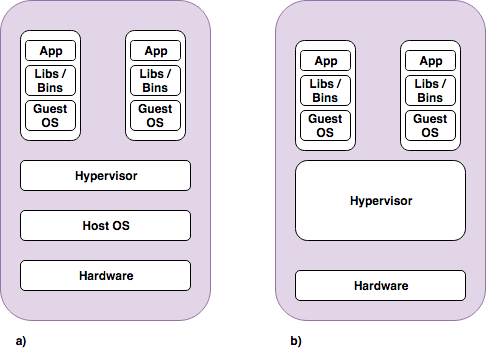
\includegraphics[width=0.7\textwidth]{difference_bare_metal_hosted_hypervisor.png}}
  \caption{Architectural differences between (a) hosted hypervisor and (b) bare metal hypervisor}
  \label{fig:hypervisor_difference}
  \end{figure}


\subsection{...To Containers}

\textit{Container-based virtualisation} represents another approach to
virtualisation, mainly spread in the last years. Compared to hypervisor-based
virtualisation it results lighter, using the host's kernel to run multiple
virtual environments. It virtualises at operating system level (it is also known
as \textit{OS-level virtualisation}) allowing other applications to run without
installing their own kernel on the host. Containers look like separated
processes that just share host's kernel and are more isolated from the host's
system (\myfig{\ref{fig:container_architecture}}). \par Resources are provided
by the host's OS together with the \textit{container engine}. A container engine
is the technology in charge of create and manage containers. \textit{Docker}
represents one of the most important and most used container engine. A computer
program running inside a container can only see the resources allocated to that
particular container. On the same host there could be more than one container,
each one with its personal set of dedicated resources. Although it could be
possible to run more than one computer program inside the same container, it is
always suggested to run only one program per container, in order to separate
areas of concern. It is better to connect multiple containers using user-defined
networks and shared volumes. Containers are particularly appreciated inside
multitenant environments for their lightness and for their approach to host's
resources sharing, which increases average hardware use.\par There are many
examples of containerisation implementations, like \textit{Linux-VServer},
\textit{OpenVZ} and \textit{LinuX Container (LXC)}. This last implementation
will be better described in the next paragraph allowing to better understand the
behaviour of containers. 

\begin{figure}[ht!]
  \centerline{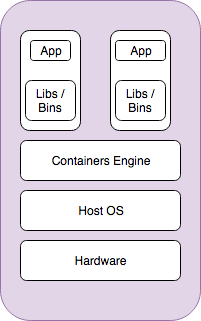
\includegraphics[width=0.3\textwidth]{container_architecture.png}}
  \caption{Architecture of a container-based virtualisation}
  \label{fig:container_architecture}
  \end{figure}

% figure of the OS virtualisation

\subsection{LXC}

\textit{LinuX Containers}, better known as LXC, are an OS-level virtualisation
technique created in 2008. They allow to run multiple isolated Linux instances
(the \textit{containers}), on top of a single \textit{LXC host}, which shares
its Linux kernel \cite{wikipedia_LXC}. Each container ``sees'' its own CPU,
memory, network interface, I/O, ... \par The isolation among containers is
obtained thanks to some Linux kernel's tools: namespace and cgroups. In the
following subsections I will analyse these two components, both for their
importance for containerisation and for the fact that they are also the basic
components in Docker.

\subsubsection{Kernel Namespace}

\textit{Namespaces} allow to create isolated environments, in which each process
that belongs to that particular environment can see global host's resources as
personal isolated resources. In other words they allow to create pool of
processes that think to be the only ones of the system. In this way groups of
processes, that are part of different namespaces, can see different set of
resources. Namespaces work by assigning to different resources the same name in
different namespaces. In the Linux kernel six different type of environments are
implemented \cite{red_hat_introduction_to_namespaces}:
  \begin{itemize}
    \item \textbf{Mount namespaces} isolate the set of file system mount points
    seen by a group of processes so that processes in different mount namespaces
    can have different views of the file system hierarchy. With mount
    namespaces, the mount() and umount() system calls cease to operate on a
    global set of mount points (visible to all processes) and instead perform
    operations that affect just the mount namespace associated with the
    container process. 
    \item \textbf{UTS namespaces} isolate two system identifiers (nodename and
    domainname) returned by the uname() system call. This allows each container
    to have its own hostname and NIS domain name which is useful for
    initialisation and configuration scripts based on these names. 
    \item \textbf{IPC namespaces} isolate certain inter-process communication
    (IPC) resources, such as System V IPC objects and POSIX message queues. This
    means that two containers can create shared memory segments and semaphores
    with the same name, but are not able to interact with other containers
    memory segments or shared memory. 
    \item \textbf{Network namespaces} provide isolation of network controllers,
    system resources associated with networking, firewall and routing tables.
    This allows container to use separate virtual network stack, loop-back device
    and process space. In this way it is possible to add virtual or real devices
    to the container assigning them their own IP Addresses and even full iptables
    rules. 
    \item \textbf{PID namespaces} allow processes in different containers to
    have the same PID, so each container can have its own init (PID1) process
    that manages various system initialisation tasks as well as containers life
    cycle. Also, each container has its unique \textit{\/proc} directory. From
    within a container only processes running inside the container can be
    monitored. The container is only aware of its native processes and can not
    ``see'' the processes running in different parts of the system. On the other
    hand, the host operating system is aware of processes running inside of the
    container, but assigns them different PID numbers.
  \end{itemize} 

\subsubsection{Cgroups}

\textit{Cgroups} are a kernel tool used to manage resources that belong to
different processes. They gather, track and limit the use of resources by
processes. It is possible to create and manage \textit{cgroups} using high level
code, assigning PID to a specific \textit{cgroup}. They represent the
fundamental tool to obtain resource isolation, playing an important role also
for the CPU and I/O's scheduling. The resources that can be limited by Cgroups
are \cite{red_hat_introduction_to_cgroups}:
\begin{itemize}
  \item \textbf{memory} - this subsystem sets limits on memory use by tasks in a
  cgroup and generates automatic reports on memory resources used by those
  tasks. 
  \item \textbf{CPU} - this subsystem uses the scheduler to provide cgroup tasks
  access to the CPU. 
  \item \textbf{CPUacct} - this subsystem generates automatic reports on CPU
  resources used by tasks in a cgroup. 
  \item \textbf{CPUset} - this subsystem assigns individual CPUs (on a multicore
  system) and memory nodes to tasks in a cgroup.
  \item \textbf{blkio} - this subsystem sets limits on input/output access to
  and from block devices such as physical drives (disk, solid state, or USB). 
  \item \textbf{net\_cls} - this subsystem tags network packets with a class
  identifier (classid) that allows the Linux traffic controller (tc) to identify
  packets originating from a particular cgroup task. 
  \item \textbf{net\_prio} - this subsystem provides a way to dynamically set
  the priority of network traffic per network interface. 
  \item \textbf{ns} - the namespace subsystem. 
  \item \textbf{devices} - this subsystem allows or denies access to devices by
  tasks in a cgroup. 
  \item \textbf{freezer} - this subsystem suspends or resumes tasks in a cgroup.
  \item \textbf{perf\_event} - this subsystem identifies cgroup membership of
  tasks and can be used for performance analysis. 
\end{itemize}   

\subsection{Docker}

As today, \textit{Docker} represents the most used computer program for
operating-system-level virtualisation (containerisation). It is developed by
\textit{Docker, Inc} \cite{docker_official_site} and it was introduced during
the 2013's PyCon conference. During its presentation \par\textit{Docker} was
announced as the future of Linux Containers \cite{docker_pycon_presentation},
indeed from its first releases it reiterated many concepts from them, such as
\textit{namespaces} and \textit{cgroups}, but providing a simpler user
experience and a complete ecosystem to create and manage containers.\par
Docker's success is mainly addressable to its portability and lightweight nature
which allow to create high density environments. It is the ideal software in
scenarios where continuous integration and continuous delivery (CI/CD) are
required, allowing developers to not only build their code, but also to test
their code in any environment type and as often as possible to catch bugs early
in the applications development life cycle \cite{docker_ci_cd}. 

\subsubsection{History}

\textit{Docker} was born as an inside project within \textit{dotCloud}, a
platform-as-a-service (PaaS) company, later renamed to \textit{Docker, Inc}.
Solomon Hyckes \cite{solomon_hyckes_wiki} was the leader of the project, that
was at first developed with other \textit{dotCloud}'s engineers, like Andrea
Luzzardi and Francois-Xavier Bourlet. The project went public, as said before,
during 2013's PyCon conference and it was released as open-source software
during the same year. Always during 2013, \textit{Docker} distanced itself from
Linux Containers, replacing them with a new execution environment (starting from
version 0.9), \textit{libcontainer}.\par \textit{Docker} represented a turning
point in the IT industry, as it can be proved by looking ad its adoption. The
following is a list from Wikipedia \cite{docker_history_wiki} of the milestones
achieved by Docker:
\begin{itemize}
  \item On September 19, 2013, Red Hat and Docker announced a collaboration
  around Fedora, Red Hat Enterprise Linux, and OpenShift.
  \item In November 2014 Docker container services were announced for the Amazon
  Elastic Compute Cloud (EC2).
  \item On November 10, 2014, Docker announced a partnership with
  Stratoscale.
  \item On December 4, 2014, IBM announced a strategic partnership with Docker
  that enables Docker to integrate more closely with the IBM Cloud.
  \item On June 22, 2015, Docker and several other companies announced that they
  are working on a new vendor and operating-system-independent standard for
  software containers.
  \item As of October 24, 2015, the project had over 25,600 GitHub stars (making
  it the 20th most-starred GitHub project), over 6,800 forks, and nearly 1,100
  contributors.
  \item A May 2016 analysis showed the following organisations as main
  contributors to Docker: The Docker team, Cisco, Google, Huawei, IBM,
  Microsoft, and Red Hat.
  \item On October 4, 2016, Solomon Hykes announced InfraKit as a new
  self-healing container infrastructure effort for Docker container
  environments.
  \item A January 2017 analysis of LinkedIn profile mentions showed Docker
  presence grew by 160\% in 2016.[30] The software has been downloaded more than
  13 billion times as of 2017.

\end{itemize}   

\subsubsection{Docker's Architecture}

\textit{Docker} follows a client-server architecture where three main components
can be distinguished \cite{docker_architecture}
(\myfig{\ref{fig:docker-architecture}}):
\begin{itemize}
  \item The server, which is a daemon process (called \textbf{dockerd}) running
  on the host's machine. It is in charge of create and manage Docker's objects.
  \item A set of interfaces conformed to REST architectural style, that enable
  programs to communicate with the server, sending instructions.
  \item A command line interface (CLI) client, that allows the user to interact
  with Docker using the REST API through their terminal. 
\end{itemize}   

\begin{figure}[ht!]
  \centerline{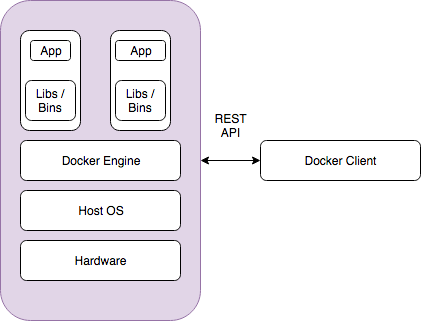
\includegraphics[width=0.6\textwidth]{docker_architecture.png}}
  \caption{Docker's architecture}
  \label{fig:docker-architecture}
  \end{figure}

\subsubsection{Docker's Components}
\label{sec:docker_object}

Docker's workflow includes the interaction with many special purpose components
created and managed by \textit{dockerd}:
\begin{itemize}
  \item \textbf{IMAGES} are the basic components involved in the creation of a
  Docker's container, they include all the instructions that the daemon has to
  follow in order to run a container. An image can be created from scratch or it
  can be based on already existing images (for example on the image of
  \textit{nginx} if we want to create a web server) where the other needed
  components are installed. \par A \textit{Dockerfile} is a special file that
  follows a very simple syntax, which includes all the steps that must be
  followed in order to create an image. Each instruction represents a layer in
  the image. When we insert a new layer (modifying the \textit{Dockerfile})
  rebuilding a container, only the new layer is rebuilt, speeding up the
  deployment's process. An image is built from a Dockerfile using the
  \textit{docker build} command. \par Another way to create an image is to run
  an already existing container, perform all the modifications needed and at the
  end save the status achieved as a new image with the \textit{docker commit}
  command.\par Docker images are stored inside registries which can be private
  or public. The two most famous public registries are \textit{Docker Cloud} and
  \textit{Docker Hub}, the latter is the default one visited by Docker for
  searching images. Developers can build their own images and upload them to the
  Docker Hub, or they can just download already existing images from it.
  Developers' images on Docker Hub are by default public, only the paid accounts
  can upload private images. These images take a standard name, that has the
  form ``developer\_uid/repository\_name''. \textit{Docker, Inc.} provides some
  official images. \par A Docker image can also contain a \textit{tag}, that is
  just an ID that conveys information about a specific image version/variant. A
  tag can be added to an image using the command \textit{docker tag}. If no tag
  is specified, the \textit{latest} tag is assigned by default.  
  \item \textbf{CONTAINERS} represent the running instances of images. The
  relationship between images and containers could be compared to the
  relationship between classes and objects in an object-oriented programming
  language like Java. A container can be connected to the network or to a
  storage and it can be defined by its image or by the configurations indicated
  starting it. A container can be launched using the \textit{docker run}
  command.\par When a container is started Docker searches locally for all the
  needed images (downloading them from online public registries if necessary),
  then a read/write file system is allocated, where the container can create or
  modifies file or directories.  By default a container can be connected to the
  external network using the host's connection. When a container is stopped  any
  changes to its state, that are not stored in persistent storage, disappear.
  \item \textbf{SERVICES} are supported from version 1.12 of Docker. Like in a
  distributed system, services represent the different pieces of an application.
  In particular in the context of Docker a service is just a running container
  in which it is defined the way that its image will be executed. Through
  services indeed a user could configure the port which a container will use,
  the number of replicas that will run of such container to better scale an
  application, ... \par The services that will run on a host can be
  configured by a special Docker file: \textit{docker-compose.yml}. This file
  contains all the instructions that must be followed to run our application's
  services. For each service indicated it specifies where to pull the
  correspondent Docker image, the port mapping between the container and the
  host, the load-balanced overlay network that will be used and all the
  information needed to deploy such service (the number of replicas, the amount
  of resources needed, the restart policy, ...).
  \item \textbf{SWARMS} are cluster composed by machines that are running
  Docker. A \textit{swarm manager} is a machine belonging to the cluster and in
  charge of executing the commands received. A user continues to run Docker
  commands normally as described before, the difference is that such commands
  are executed by the swarm manager, which decides how to run these commands
  (for example filling the host with less running containers or assigning to
  each host one instance of the specified container). In a cluster there could
  be more than one swarm manager. \textit{Workers} are machines belonging to the
  swarm, but without the same privileges of a swarm managers. They just provide
  more computational capacity to the cluster. In general all the machines inside
  a Docker swarm are referred as \textit{nodes}.
\end{itemize}
%%% TODO: capabilities

\subsubsection{Common Usage Of Docker}

As stated in the previous paragraphs, Docker's success is mainly attributable to
its simplicity of use and to its ``lightness''. Such characteristics have
increased its adoption among developers and organisations. John Willis, a
Technical Evangelist at Docker, during an interview
\cite{ibm_interview_john_willis} for the IBM Infrastructure Blog stated that the
most common use cases for Docker are mainly three:
\begin{itemize}
  \item \textit{Integration test}: With virtual machines running integration
  test could take also days. The virtual machines should be configured and
  installed, then after the tests they should also be rebase back to their
  original state. On the contrary with Docker the configuration and the
  execution of a containers takes less time and also rebase could be done in few
  seconds.
  \item \textit{Immutable delivery model}: With Docker when a developer needs to
  commit its code he can just commit a Docker image. In such a way the software
  tested on his own computer will be the same identical software which will run
  in production. This principle allows to speed up the deployment process, not
  requiring further configurations to run the software on the production hosts.
  \item \textit{Container as service}: Docker allows to build up a collection of
  pre-built binaries (Docker images) that can be shared, for example pushing
  them into the Docker Hub. In such a way an organisation can speed up its
  production and also increase its set of used tools, not needing to set up its
  own tools but just to pull new images.
  
\end{itemize}

\newpage

\section{Docker's Security Threats}
\label{sec:docker_security_threats}
 
In this section I analyse the most important security threats for a Docker
system. For each possible threat I describe its characteristics and how it could
be possible to take advantage of it. I also provide a practical example of an
attack which exploits the vulnerability described, exception made for those
threats that are more generic, not regarding specifically Docker containers.
\par In the next section I will start from these security threats in order to
define the best practice to follow using Docker.

\subsection{Analysis Of Docker Security Threats}

In order to list the main security threats that afflict a Docker system, I
started from a possible definition of the attack surface for the Docker
containers. I have analysed a series of studies present in literature, from
Yasrab's paper ``Mitigation Docker Security
Issue'' \cite{mitigating_docker_security_issues_yasrab} to  ``To Docker or Not to
Docker: A Security Perspective'' written by Combe, Martin and Di
Pietro \cite{to_docker_or_not_to_docker}, through Sysdig's list of the well known
vulnerabilities of Docker \cite{sysdig_docker_vulnerabilities}. Finally, I have
divided the Docker attack surface in five macro areas:
\begin{itemize}
  \item \textit{Isolation}: The most important difference between a normal
  process running on a host and a Docker container is the degree of isolation of
  the latter. As seen in the previous section, Docker uses different Linux
  kernel features to achieve an optimal isolation. However, such tools must be
  well configured, because it is possible that their default behaviour leads to
  \textit{denial-of-service attacks}, \textit{container breakouts} or
  \textit{ARP spoofing attacks}.
  \item \textit{Host Hardening}: Docker containers share the kernel with the
  host making them lighter than a virtual machine. Such characteristic increases
  the importance of the host's kernel security, cause both the containers and
  the host depend on it. \textit{Kernel exploits}, for example, can lead to
  malfunctions of both the host and the containers. 
  \item \textit{Image Security}: Docker images are fundamental for the correct
  execution of Docker containers. If a \textit{poisoned image} is downloaded and
  used, an attacker can compromise the entire system. In the same way the use of
  \textit{outdated Docker images}, can lead to bugs in the system easily
  exploitable by attackers. For this reason, maximum precaution must be taken
  managing Docker images.
  \item \textit{Erroneous Configurations}: Docker has made of its simplicity of
  use its most important feature. However some precautions must be taken
  configuring a Docker system. For example an \textit{erroneous management of
  the secrets} can bring to an impairment of the system. 
  \item \textit{Running Container}: Inside a Docker container there is anyway
  our running program. All the bugs and vulnerabilities that afflict our program
  can be used by an attacker to hit our system. For this reason, to cover all the
  attack vectors of our Docker containers, we should also \textit{monitor the
  runtime activities of our containers}.
\end{itemize}
From these macro areas, I have extracted eight security threats for Docker
containers, analysing them in the following paragraphs.
 
\subsubsection{Kernel Exploits}

One of the main advantages of container-based virtualisation, so of Docker,
is that the host shares its kernel with all the running containers. In this way
this kind of virtualisation results lighter than an hypervisor-based one,
avoiding the overhead of installing the guest's kernel. As we will see this is
on the one hand a big advantage in terms of speed and efficiency, but on the
other hand it represents a big threat for the security of the system. The host's
kernel, indeed, handles all the operations of the containers, so in case of a
\textit{kernel-level exploit} all the containers that are running on the system
are at risk of being compromised.\par Kernel exploits can be done by an attacker
who takes advantages of a bug or a vulnerability of the kernel. In this way he
can run his software in kernel mode, manipulating processes' privileges and
bringing him to take control of the system. If such exploit is performed inside
a container, it has consequences also on the host OS. In particular if the
attack allows the attacker to execute his code, this execution will happen on
the host OS, not inside the container; in the same way if the attack allows to
read arbitrary memory, so the attacker could read and write memory parts that
belong to other containers.\par Kernel exploits are also a security threat in
the context of an hypervisor-based virtualisation, but in that case the attack
would result more complicated. Indeed the attacker should be able to exploit the
VM's kernel, the hypervisor and the host's kernel. While on a container-based
virtualisation it is sufficient to exploit the only host's kernel.

\bigbreak\textbf{Practical Example}\bigbreak 

In literature there are many examples of kernel exploits used to obtain control
over an entire system. In this paragraph I will focus on \textit{Dirty COW}, an
attack that takes advantage of a privilege-related vulnerability in order to
allow the attacker to gain high privileges on the system. The official reference
to this bug is CVE-2016-5195.\par It exploits a race condition inside the Linux
kernel's memory subsystem that handles the copy-on-write (COW) mechanism, in
this way an unprivileged user could gain write access to a read-only memory part
\cite{red_hat_dirtycow}.\par In order to obtain this exploit, we must create a
loop involving two threads:
\begin{itemize}
  \item one thread tries to access inside a read-only memory location to
  write, creating in this way a modified copy inside the process's memory
  \item another thread, calls the syscall \textit{madvise()}
  \cite{madvise_description} with the MADV\_DONTNEED parameter (such parameter
  indicates that is not to be expected to access the memory location in
  question) for the newly allocated memory
  \end{itemize}
The simultaneous execution of these two threads in a loop could bring the
kernel to point to the modified copy of a file in memory that should instead be
read-only \cite{dirtycow_how_it_worrks}.

\subsubsection{Denial-of-service}

As we have seen for kernel exploits, the fact that all the containers running on
a host share the same kernel can be both positive and negative at the same time.
All the containers, indeed, share also the same resources and if the access to
them is not limited in some way one container could require a huge amount just
for it, bringing the host and the other containers to starvation. This type of
attack is known as \textit{denial-of-service(DoS)}.\par Denial-of-service
attacks are very well-known attacks in literature, especially in multi-tenant
systems, that are the ones where Docker is mostly used.  The aim of the attack
is to make a system or a network resource unavailable. It is typically
accomplished by flooding the targeted machine or resource with superfluous
requests in an attempt to overload systems and prevent some or all legitimate
requests from being fulfilled \cite{dos_wikipedia}. An attack of this genre,
conducted against a Docker container, brings to unavailability not only the
container itself, but also the host where it is virtualised together with all
the other system's containers.\par On a virtual machine this type of attack is
also possible, but it is more difficult to be completed. This is due to the fact
that the hypervisor is configured to restrict its use of resources. For a
container, instead, resources management is defined at application layer.\par In
the previous section we have seen how Docker has inherited cgroups from LXC to
allocate resources needed by containers. However, as described on Docker's
documentation \cite{resource_on_docker}, this kernel tool is not enabled by
default, so a container can use as much of a given resource as the host's kernel
scheduler allows. We will see in the next section how to configure Docker to
work with cgroups, managing resources for containers. 

%\bigbreak\textbf{Practical Example}\bigbreak 

\subsubsection{Container Breakout}

If a user inside a Docker container bypasses all the isolation checks,
``escaping'' from the container, it would have direct access to the host and to
all the other containers in the system. This situation can be achieved using an
exploit or a not correct configuration of the Docker environment. Such type of
attack is known as \textit{container breakout}.\par This type of vulnerability,
according to Docker website \cite{docker_blog_about_container_breakout}, was
mitigated with Docker 1.0, nevertheless a not trusted program running with root
privileges inside a Docker container could still represent a source of risk.
\par Container breakout is mostly possible in situations where privileges inside
a container were not properly configured. By default, users are not namespaced,
so any process that breaks out of the container will have the same privileges on
the host as it did in the container. A root user in a container will also be
root on the host. Moreover, in the earliest versions of the Docker engine, some
specific kernel capabilities were dropped, but still leaving some important ones
granted. From Docker 1.0, instead, a different approach was taken: all the
capabilities were dropped, except some necessary, giving the user the
possibility to decide which one to allow. De facto this newly approach
transformed the use of capabilities from a blacklist to a white-list.

\bigbreak\textbf{Practical Example}\bigbreak 

One of the most famous container breakout exploit is 2014's \textit{Shocker}
\cite{shocker}. I will analyse such attack with the aim to demonstrate how a
Docker container can access some privileged file-system data when Linux
capabilities are not managed carefully.\par Shocker takes advantage of the
\textit{CAP\_DAC\_READ\_SEARCH} capability, that was granted by default to a
superuser inside a container with a version of Docker prior to the 1.0. This
capability is the one which allows to use the system call
\textit{open\_by\_handle\_at()}, conceding to access a file on a mounted
file-system through a file\_handle structure. A file\_handle is quite different
than a file descriptor, because it can be generated inside a process using
\textit{name\_to\_handle\_at()} and then recalled by another process with
\textit{open\_by\_handle\_at()} (while a file descriptor can't be properly
passed between different processes). In this way if a process has an handle
opened for a host's file or a different container's file and our container has
not the privileges to access it, we can still call
\textit{open\_by\_handle\_at()} on the opened handle
\cite{shocker_how_it_works}.

\subsubsection{Poisoned Images}

As said in \ref{sec:docker_object}, Docker images represent one of the most
fundamental building blocks for a container. If an attacker obtains to make his
images to run, the host and all its containers are seriously at risk. \par
Container images are claimed to be downloaded and verified by default by Docker,
thanks to the presence of a signed manifest inside the image. In such mechanism
however Docker does not verify the image's checksum from the manifest. In this
way an attacker could provide his \textit{poisoned images} with some virus,
together with a signed manifest. \par Docker fetches and unpacks a container
image in just one step without verification, using the command \textit{docker
pull}. Jonathan Rudenberg explained in a post \cite{docker_image_insecurity} on
his blog how the process of downloading a Docker image can be extremely
insecure. Images are downloaded using HTTPS, but then they go immediately
through a processing pipeline inside the Docker daemon:
\bigbreak\centerline{decompress $\,\to\,$ tarsum $\,\to\,$ unpack}\bigbreak This
pipeline, even if it is functional, is insecure. The reason lies in the fact
that the not trusted input is processed before its verification. A compromised
image does not need to run to lead to malfunctions of the system. As stated by
one blog post from Red Hat \cite{docker_pull_red_hat}, an attacker can
compromise the system even during the unpack step. For example an issue (now
solved) exploited a tarball's capacity to perform directory traversal attacks,
allowing compromised images to override parts of a host file system.

\bigbreak\textbf{Practical Example}\bigbreak 

CVE-2014-9357 \cite{CVE-2014-9357} is a known vulnerability, solved from Docker
1.3.3, that allowed attackers to execute arbitrary code with root privileges via
a malicious image or a build from a compromised Dockerfile. Such vulnerability
exploited the fact that \textit{xz} utility, used for decompressing LZMA
archives during a call to \textit{docker pull}, was executed as root. 

\subsubsection{Outdated Images}

The importance of images in Docker ecosystem makes it of primary importance to
attest their security. On the one hand we have seen how images could be
\textit{poisoned} by an attacker, on the other hand even if our images are not
compromised it does not mean that they are safe. It is important to make
sure that the images at the base of our running containers are updated, not
containing any known vulnerabilities.  An outdated image can be affected by a
series of security threats that were already fixed in an updated version of the
same image. \par A study by Gummaraju, Desikan, and Turner at BanyanOps
demonstrated how about more than the 30\% of the official repositories present
on Docker Hub are affected by a variety of security threats, such as
\textit{heartbleed}, \textit{shellshock}, \textit{poodle}, ... These numbers
grow up to the 40\% taking in consideration also the images loaded by users
\cite{gummaraju_desikan_turner}. 

\subsubsection{Management Of Secrets}

Docker containers are very used in the development of microservices. A
microservice architecture is very different than a monolithic one, specially in
the deployment phase: a monolithic architecture is often just configured,
launched and then it runs for a long period of time (which could even last
years); microservices are continuously created and destroyed. In both cases,
sensitive information are needed, like API keys, database passwords, SSL/TLS
keys, SSH keys, ... Compromising these information would compromise the entire
system. \par In a monolithic architecture the management of these information is
non trivial, indeed they can be stored in the system permanently and the can be
renovated using some mechanism like the ``Privileged Accounts Managers''
\cite{privileged_accounts_managers}. Despite these solutions have been used and
tested for years in the context of monolithic service, they can't be applied to
microservices based on containers. The two main concerns for the management of
secrets inside Docker containers are \cite{secret_management_concerns_docker}:
\begin{itemize}
  \item Docker images have an immutable nature, this means that they are created
  once and then deployed in many different environments. Their nature is
  strongly in contrast with the idea of saving secrets directly inside them.  
  \item Requesting such secrets at runtime imply performing a prior
  authentication procedure, but this procedure is difficult to be implemented
  without storing some secrets for the authentications itself.
\end{itemize}
The use of environment variables is highly discouraged, due to the fact that
these variables can be easily leaked. They are indeed exposed in too many
places, like child processes, linked containers and \textit{Docker inspect} (a
tool provided by Docker for retrieving low-level information on the used
objects).\par All these reasons make \textit{management of secrets} a central
topic in the discussion of Docker's security. 

\bigbreak\textbf{Practical Example}\bigbreak 

One example of how a bad management of secrets could be fatal for an agency
comes from IBM. In 2017 a privilege escalation vulnerability was found inside
IBM Data Science Experience, that is a data analytics product
\cite{ibm_data_science_experience}. Such vulnerability was caused by a wrong
configuration of the Docker containers that were running the service. IBM's
engineers left inside the containers Docker TLS keys, leaving root access across
the whole computer cluster and read/write access to terabytes of sensible
customer data. \par As stated by the report of the vulnerability
\cite{ibm_data_sciene_report}, an exploit of such threat was also quite easy,
needing only an access to to Internet and a web browser:
\begin{itemize}
  \item The attacker should just enter the service's web environment, accessing
  to its command line
  \item He should download and extract the Docker binary of the service, using
  the following commands: 
  \begin{lstlisting}[language=bash,breaklines]
    system("wget https://test.docker.com/builds/Linux/x86_64/docker-1.13.1-rc1.tgz")
    system("wget https://test.docker.com/builds/Linux/x86_64/docker-1.13.1-rc1.tgz")
  \end{lstlisting}
  \item He should use the downloaded Docker binary with the existing
  certificates to achieve root access to the host mounted volume:
  \begin{lstlisting}[language=bash,breaklines]
    system("DOCKER_API_VERSION=1.22 ./docker/docker -H 172.17.0.1 \
              --tlscacert /certs/ca.pem --tlscert /certs/cert.pem \
              --tlskey /certs/key.pem \
              run -v /:/host debian cat /host//shadow")
  \end{lstlisting}
\end{itemize} 

\subsubsection{ARP Spoofing}

Inside an host, all the containers, if not properly configured, can communicate
with each other through their network interfaces. Docker uses namespaces to
create an independent network stack for each container, giving them their own
own IP addresses, IP tables, ... By default Docker provides connectivity between
the containers creating a Virtual Ethernet Bridge, named \textit{docker0}. At
container creation time, Docker creates and connect a new network interface with
a unique name to the bridge. Such interface is also connected to the
\textit{eth0} interface of the
container(\myfig{\ref{fig:docker_network_model}}). This type of configuration is
vulnerable to \textit{ARP spoofing} attacks, since the bridge forwards all of
its incoming packets without any filtering. \par An ARP spoofing attack is a
very well known attack in literature. It takes advantage of the ARP protocol,
which doesn't provide a basic method to authenticate ARP messages. In order to
perform such type of attack, the attacker must be connected directly to the
target LAN with his machine or to a compromised host that belongs to the
network. In the case of Docker, such conditions is satisfied if the attacker
manages to compromises a container running on a host: in this way he would have
access to the local network between all the containers running on the host. The
main goal of this type of attack is to divert traffic directed to a container to
the compromised container controlled by the attacker.   
\begin{figure}[ht!]
  \centerline{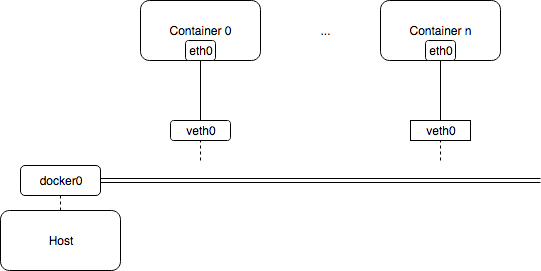
\includegraphics[width=0.7\textwidth]{docker-network-model.png}}
  \caption{Docker default network model}
  \label{fig:docker_network_model}
  \end{figure}

\bigbreak\textbf{Practical Example}\bigbreak 

A practical example of this type of attack can be reproduced inside a
containerised environment just running a Docker container with \textit{dSniff}
installed. Dsniff is a set of password sniffing and network traffic analysis
tools, which contains among others also \textit{arspoof}, a tool used
specifically to perform ARP spoofing attack \cite{wiki_dsniff}. \par Such type of
experiment is described by Philipp Bogaerts in one of his blog post
 \cite{bogaerts_arpspoof}. He shows how it is simple to perform an ARP spoofing
attack running three containers on the same host, without changing the default
network configuration:
\begin{itemize}
  \item Two containers are created just from the Busybox base image, running the
  ``ifconfig'' command on each in order to read their IP address. We will call
  these two containers just \textit{container\_0} and \textit{container\_1}.
  \item One container, which will be the one that performs the attack, is created
  starting from the Debian base image, to which it is installed only dSniff. 
\end{itemize}
One of the first two containers ping the other, while the attacker's container
performs the attack using arspoof:
\begin{lstlisting}[language=bash,breaklines]
  arpspoof -i eth0  -t ip_container0 ip_container1 &
  arpspoof -i eth0  -t ip_container1 ip_container0 &
\end{lstlisting}
In such a way all the traffic generated between the first two containers will
pass through the attacker's container.

\subsubsection{Dynamic Aspects of Docker Security}

All the threats analysed in the former sections regard the launch-time of
containers. Kernel exploits, denial-of-service, container breakouts, ... are
all security threats that can be faced before running our containers. We can
refer to these as \textit{static aspects} of Docker security. Such threats, as
we will see in the next section, can all be mitigated following some precautions
during the creation of the images that we will run, using special configurations
and ad-hoc policies or tools.\par However container's attack surface is not
limited to such aspects, we must also consider:
\begin{itemize}
  \item All the possible vulnerabilities of the application that we want to run
  inside a container, that can be exploited by an attacker
  \item All the attacks that can be performed on a vulnerability already
  discovered but not yet patched (these attacks are also known as zero-day
  attacks)
\end{itemize}
Such attacks can not be avoided at launch-time, but they must be mitigated at
runtime, monitoring containers' activity . We can refer to them as
\textit{dynamic aspects} of Docker Security. 

%\subsubsection{Summary}

%All the attacks listed above are summarised in Tab. 1. In the next section I
%will provide a list of best practices to follow using Docker in order to prevent
%such threats. For this reason in the following table each attack is associated
%with a code, that will be reused in the next section to associate to each best
%practice the attack that it prevents.

%\begin{table}[ht]
%  \begin{tabular}{ | l | l | p{5cm} |}
%  \hline
%  Code & Threat & Practical Example \\ \hline
%  T1 & Kernel Exploit & test \\ \hline
%  T1 & 11C & test \\ \hline
%  T1 & 11C & test \\ \hline
%  T1 & 11C & test \\ \hline
%  T1 & 11C & test \\ \hline
%  T1 & 11C & test \\ \hline
%  T1 & 11C & test \\ \hline
%  T1 & 11C & test \\ 
%  \hline
%  \end{tabular}
%  \caption{Lorem Ipsum}
%  \label{table:docker_threats}
%\end{table}


\newpage

\section{Best Practices For Docker Deployment}
\label{sec:best_practices_for_docker_deployment}

As seen in the previous section, the ease of use of Docker actually hides a
series of security threats. In this section I will start right from these
security threats previously analysed in order to list several best practices
that can be followed during the deployment of Docker containers. The aim of
using such practices is to increase the security of a Docker system, trying not
to complicate the Docker user experience. Most of the practices that I will
introduce refer directly to specific attacks previously described, others are
generic practices that can be useful for increasing the security of the system.
\par The suggested tools are almost always either provided by Docker itself or
they are open-source and free, I deliberately avoid to propose commercial and
closed-source software because they are often more difficult to analyse and
test. Most of the practices are present in literature or directly suggested in
the Docker's documentation. In particular I have often referred to Gianluca
Arbezzano's ``Docker Security - Play Safe'' \cite{arbezzano_play_safe} and to
Adrian Mouat's ``Using Docker. Developing and Deploying Software with
Containers'' \cite{mouat_using_docker} to find the best practices for security
enhancement in Docker. 

\subsection{Mandatory Access Control}

A \textit{mandatory access control or MAC} system is a set of rules that define
what a subject can or can not do in reference to a certain object. Usually the
operating system plays the role of the policy administrator, while threads and
processes are the subjects and files, directories, network ports, ... are the
objects of the defined policies. When a subject tries to perform an action on an
object the OS checks all the defined policies and decides if the action can be
done or not. A user can not override or modify these policies, only the policy
administrator can \cite{wiki_MAC}. Linux uses by default discretionary access
control (DAC), restricting access to objects based on the identity of subjects
and/or groups to which they belong (authorisations are indicated on each
file/directory by the \textit{rwx} flags). MAC and DAC can works together on a
Linux machine, with DAC that must be passed before MAC evaluation \par Linux
offers some kernel security modules, like \textit{Security-Enhanced Linux
(SELinux)}, \textit{AppArmor} and \textit{Secure Computing Mode (seccomp)}, that
can be configured using access control security policies to implement mandatory
access control. Docker supports by default these modules and by using them we
can have an additional extra layer of security, which can result decisive to
mitigate kernel exploits and container exploits. An example of this can be found
in Jon-Anders Kabbe's work ``Security analysis of Docker containers in a
production environment'' \cite{kabbe_security_docker}, where he demonstrates how
Dirty COW, the kernel exploit analysed in the previous section, can simply be
prevented using Docker's default profile of AppArmor. \par  The general policy
of Docker's default profiles for the described Linux kernel security modules is
usually to protect the host from the containers and not also containers from
other containers \cite{to_docker_or_not_to_docker}. However writing specific
profiles for each container running on the system can address such problems,
making MAC very useful for the enhancement of containers isolation and for the
prevention of kernel exploits and container breakouts. 

\subsubsection{SELinux}

\textit{Security-Enhanced Linux}, better known as SELinux, is a Linux kernel
security module created in 2003 and used to develop a mandatory access control
system. With SELinux each component of our operating system has a \textit{label}
(SELinux is often known as a labelling system): process, files, directories,
devices, network port, ... are all labelled. To achieve mandatory access control
we have to write rules that control the access of a subject label on an object
label. By default everything is deny, writing policies we can allow what we
need. \par The use of SELinux with Docker allows to create access policies that
can increase containers isolation. To run Docker with SELinux we must at first
install such kernel module on our host, then we have to assign labels
accordingly to the policy that we want to create. Docker has to be launched
with the \textit{--selinux-enabled} flag to start in order to use SELinux. \par
SELinux is a very powerful tool that allows to have a great control over the
system, through its high granularity access policies and all its many
configurations. At the same time its fine-grained policy maker system makes it
very difficult and complex to maintain. For this reason other MAC tools are
often preferred.

\subsubsection{AppArmor}

\textit{AppArmor} is another Linux kernel security module based on mandatory
access control like SELinux. It offers the possibility to restrict programs'
capabilities with per-program profiles. The system administrator can create and
load a security profile into a single program, this makes AppArmor simpler to
use than SELinux and this is often the reason why it is preferred over it.
AppArmor can be used in two different modes:
\begin{itemize}
  \item \textit{Enforcement mode}, where the defined policies are followed and
  the access restricted according to them; 
  \item \textit{Complain/learning mode}, where the defined policies are not
  followed, but each violation is logged for debugging.
\end{itemize}
We can load our pre-configured AppArmor profile with Docker at launch time, if
our host supports such kernel security module. The profile is loaded directly
into the container in enforcement mode. If no profile is specified Docker uses
its default one, which denies the access only to few filesystems on the host
\cite{bui_docker_security}. AppArmor profiles are simple text files where rules
for capabilities, networking and access to certain objects can be specified.
Such rules can be referred to various access controls, denying or allowing a
subject to perform certain actions on an object.   Security profiles can be
saved in /apparmor.d/ and they can be loaded into a container using the flag
\textit{-security-opt=``apparmor:profile\_name''} with the Docker run command. 

\bigbreak\textbf{LiCShield}\bigbreak 

\textit{LiCShield} \cite{licshield} is an open-source tool that generates
AppArmor profiles by following the behaviour of the Docker daemon during the
execution of the build and run commands. The tool was presented at first only
for LXC with the paper ``Security hardening of Linux containers and their
workloads'' \cite{licshield_paper}, then it was adapted to work also with
Docker. \par LiCShield works starting from a given Docker image, it traces the
execution of the related container, collecting the information about the
performed operations, the resources used and the required permissions. From the
information retrieved LiCShield generates at the end a specific AppArmor profile
for the analysed container. 

\bigbreak\textbf{Bane}\bigbreak 

\textit{Bane} \cite{bane_jesse_frazelle} is an open-source tool created by
Jessie Frazelle, a former Software Engineer at Docker Inc., with the aim to
simplify and speedup the creation of AppArmor profiles. It basically generates
AppArmor profiles from YAML specification files. Such YAML files follow a very
simple syntax where three sections are present:
\begin{itemize}
  \item \textit{File system}, where we can define the type of actions that can be
  performed on a certain path. Actions include ``Read only'', ``Log on write'',
  ``Allow execution'', ``Deny execution'', ``Write'', ...
  \item \textit{Capabilities}, where a whitelist of the allowed capabilities is
  defined. 
  \item \textit{Network}, where allowed protocols and network policies are
  defined.
\end{itemize}
Bane directly installs the generated profiles inside AppArmor's directory.  

\subsubsection{seccomp}

\textit{Secure Computing Mode}, better known as seccomp, is a Linux kernel security
module that acts as a firewall for system calls. Writing a profile for seccomp
it can be possible to restrict the use of syscalls using a whitelist approach.
Docker's default profile for this feature disables around forty system calls,
not allowing a container to call them, restricting its privileges. It is
possible to write specific security profiles for our containers, however such
practice is discouraged due to the difficulty to write and maintain seccomp's
profiles. seccomp's profiles can be used within a container using the flag
\textit{-security-opt=``path\_to\_seccomp\_profile''} with the Docker run command.

\subsection{Host Hardening}

As well as for mandatory access control tools described in the previous
paragraph, there are many other security systems that can be used to harden a
Docker host. Such systems don't require Docker-specific configurations and can
work without interfering with other Linux tools used by default by Docker, like
capabilities. \par In this paragraph I analyse \textit{grsecurity}, one of the
most famous and known set of  patches for the Linux kernel which emphasises
security enhancements.  

\subsubsection{grsecurity}

\textit{grsecurity} \cite{wiki_grsecurity} is a collection of security features
for the Linux kernel. It is developed by open-source Security and it can be used
only by its paid subscribers, despite being free from 2001 (when it was first
released) to 2005.\par grsecurity offers different components that add safety
checks, useful to defeat many exploits. Among these components the most
important are:
\begin{itemize}
  \item \textit{PaX} \cite{wiki_PAX}: It is used for implementing least
  privilege protections for memory pages and for reducing the risk of memory
  corruption bugs. PaX provides hardening with different tools: 
  \begin{itemize}
    \item Executable space protections: It prevents those attacks
    where malicious code is inserted into the address space of a process and
    then launched. Such attacks exploit the fact that Linux by default allows
    programs to change their memory protection. On the contrary PaX denies
    memory mappings to be altered from their initial state, in this way a memory
    portion can not be executed after being written by an user. 
    \item Address space layout randomisation (ASLR): It is used to randomise the
    memory map of a process. In this way every time that a process is launched
    its memory map is different. Such mechanism prevents an attacker from
    finding its malicious code within an address space.
    \item Miscellaneous memory protections: PaX has different features used to
    protect memory, like: erasing the stack before returning from a system call;
    preventing overflows from various object reference counters; enforcing  the
    size of heap objects when they are copied between the kernel and the
    user's address space; ... 
  \end{itemize}
  \item Role-based access control (RBAC): It is a set of rules to achieve access
  control through the definition of a series of roles. Each subject of the
  system has a proper role among with its restrictions on what it can do or not
  do. The aim of role-based access control is to have roles with the absolute
  minimum privileges to work correctly and nothing more. In this way it is more
  difficult for an attacker to take control of the system and to access
  sensitive data.
  \item Chroot restrictions: They reduce the possibility of privilege escalation
  attacks arising from the use of the system call \textit{chroot}. Such
  restrictions include several prohibitions that deny the possibility to
  attach shared memory outside chroot, to send signals by fcntl outside chroot,
  to view any process outside chroot, ...
  \item Audit tools: They allow to have a complete log of specific group of
  users. In particular they can be used to log calls to \textit{chdir},
  mounting/unmounting of devices, changes to the system time and date, failed
  \textit{fork} attempts, ...
  \item Trusted path execution: It restricts the use of binaries not owned by
  the root of the system, in this way an attacker can not execute his malicious
  code.
\end{itemize}

\subsection{Management Of Secrets}

As described in the previous section, we can not manage secrets in Docker as we
do with the classic monolithic web service. They can not be stored in a
Dockerfile or in our application's source code. In this paragraph we will see a
series of tools that can be used to achieve a correct management of the secrets.

\subsubsection{Docker secrets}

\textit{Docker secrets} \cite{docker_secrets} was released with version 1.13 of
Docker. It can be used with Docker swarms to create a central built-in security
database, where secrets can be stored and transmitted to only those containers
that need access to them. Secrets are encrypted both during their transmission
and at rest inside a Docker swarm. \par When a secret is added to a Docker swarm
a bidirectional TLS connection is created between it and the swarm manager. The
secret is at first encrypted and stored inside the swarm manager, then it is
replicated among all the the other managers of the cluster to ensure its
availability. A node of the cluster can require a secret only if it is a manager
of the swarm or a running service task which have been granted access to the
secret. When the secret is transmitted to a node that requires it, it is
decrypted and stored inside the container in an in-memory file system. When the
node stops running its stored secrets are unmounted and flushed from the
container's memory.\par A secret can be added to Docker using the command
\textit{docker secret create secret\_name *secret*} and the it can be included
inside a container using the flag \textit{--secret secret\_name} with the Docker
run command.

\subsubsection{Vault}

\textit{Vault} \cite{hashicorp_vault} is a tool developed by HashiCorp for
securing access to secrets. It can save secrets to disk or to other persistent
services, including also Hashicorp's own backend system
\textit{Consul} \cite{hashicorp_consul}.\par Vault offers different features that
can be useful in order to achieve a correct and secure management of secrets:
\begin{itemize}
  \item Secrets are encrypted before being written to a persistent storage. In
  this way an attacker that achieves to access to the storage can not
  obtain secrets anyway. 
  \item Each secret has an associated lease. An user can renew such lease using
  Vault's API. At the end of the lease Vault process to revoke the associated
  secret.
  \item Secrets can be generated and revoked dynamically for some of the most
  used web services, like AWS or SQL databases. When an application needs to
  access to one of these services Vault generates a keypair with valid
  permissions on demand. At the end of the lease the keypair will be revoked
  automatically from Vault itself.
  \item In case of key rolling or of a detected intrusion in the system, Vault
  is able to revoke entire tree of secrets. For example all the secrets
  accessed by a user or that belong to a specific category.
\end{itemize}
\par As stated Vault can use Consul as backend, they can be used by a process
inside a Docker container for managing secrets and they can also be deployed as
Docker containers themselves. Vault can be initialised from its container using
the \textit{init} command, which creates a file with the information to access
the vault. Such information contain five master keys and an access token that
should  be stored separately and securely offline or using a third-party
service. Vault starts at first in a \textit{sealed} state, in which it can
communicate with the backend but it can not decode the contents retrieved. To
decode the data we must go through a \textit{unsealing} process. During such
process three of the five master keys previously generated must be provided to
the Vault process, using the \textit{unseal} command. Finally to access to Vault
for reading and writing data the access token must be used to authenticate.  

\subsection{Resource Limitation}

Denial-of-service attacks can be a serious threat for Docker containers as we
have seen in the previous section. In order to prevent such attacks we must make
sure that the use of resources by containers is limited. Docker provides its own
ways \cite{resource_on_docker}, based on the use of cgroup, to manage
how much memory, CPU, or block IO a container can use.

\subsubsection{Memory Limitation}

Docker offers two possibilities for limiting the use of memory: \textit{hard
limit} and \textit{soft limit}. The former allows to indicate the maximum amount
of memory that a container container can use; the latter allows a container to
use as much memory as it needs until Docker detects contention or low memory on
the host machine. \par Memory limitation can be set using runtime configuration
flags of the \textit{docker run} command: 
\begin{itemize}
  \item \textit{-m or --memory=} indicates an hard limit to the amount
  of memory that a container can use.
  \item \textit{--memory-swap} can be used if an hard limited has been set. It
  indicates how much memory a container is allowed to swap to disk. If a
  positive number is indicated, it represents the total amount of memory and
  swap that can be used. If the indicated number is equal to the one specified
  as hard limit, the container can not access to swap. By default (if this flag is
  unset) the container can access twice as much swap as the hard limit indicated.
  \item \textit{--memory-reservation} indicates a soft limit to the amount
  of memory that a container can use. If this flag is used in combination with
  an hard limit, the amount of memory specified must be lower than the one
  indicated with the \textit{--memory} flag.
\end{itemize}
An integer number must follow such flags to indicate the amount of memory,
together with one of the following suffix: \textit{b} (bytes), \textit{k}
(kilobytes), \textit{m} (megabytes), \textit{g} (gigabytes).
  
\subsubsection{CPU Limitation} 

Docker allows to set different constraints in order to limit a container's
access to the host's CPU. As for memory also CPU limitation can be set using
runtime configuration flags of the \textit{docker run} command:
\begin{itemize}
  \item \textit{--cpus=\textless value \textgreater} indicates the amount of CPU
  resources that a container can use. The value indicated is proportional the
  number of CPUs that a host has. 
  \item \textit{--cpuset-cpus} indicates the specific CPUs or cores that a
  container can use. An hyphen specifies a range (for example 0-2 indicates to
  use from the first to the third CPU/core), while a comma indicates a list
  (0,2 means to use the first and the third CPU/core).
  \item \textit{--cpu-shares} assigns a \textit{weight} to a container  when CPU
  cycles are constrained. A weight is used to prioritise container CPU resources
  for the available CPU cycles. The default weight for a container is 1024.
\end{itemize}

\subsubsection{I/O Limitation}

As seen for memory and CPU, Docker can limit also I/O for a container. The
runtime configuration flags that can be used are: 
\begin{itemize}
  \item \textit{--device-read-bps} indicates the limit (in bytes per second)
  with which a container can read from a device.
  \item \textit{--device-read-iops} indicates the limit (in IO per second)
  with which a container can read from a device.
  \item \textit{--device-write-bps} indicates the limit (in bytes per second)
  with which a container can write to a device.
  \item \textit{--device-write-iops} indicates the limit (in IO per second)
  with which a container can read to a device.
\end{itemize}

\subsection{User Namespace}

Most of the privilege-escalation attacks can be prevented running Docker
containers' application as unprivileged user. At the same time, however, some
applications require explicitly to run as root within their containers. In these
cases it can be useful to \textit{remap the root user} \cite{isolate_namespace}
of a Docker container to a less privileged user on the Docker host. Such
technique is possible thanks to the use of Linux namespaces. \par The namespace
remapping is achieved through two important files: \textit{/etc/subuid} and
\textit{/etc/subgid}. These files contain an entry for each user in the system
and each entry is composed by three fields that represent: the ID of a user, his
beginning UID (in /etc/subuid) or GID (in /etc/subgid) and a maximum number of
UIDs or GIDs available to the user. \textit{dockermap} is the default ID used by
Docker to represent the unprivileged system user that is used for the remapping.
We can manually create this entry inside the two files, specifying an arbitrary
range for the UID/GID (paying attention to not overlap the range of the new user
with the already existing ranges of the other host's users). At this point we
can configure the Docker daemon to run containers using the just created user.
To do this we can edit Docker's JSON configuration file
\textit{/etc/docker/daemon.json} appending the option: \textit{``userns-remap'':
``default''}. \par It is important to pay attention to the fact that if there is any
location on the host where a container can write, permissions must be
adjusted accordingly for the dockermap user. 

\subsection{Image Creation}

Creating our Docker images is an important aspect in the use of Docker. Follow
some basic rules during this process can be fundamental for our system in terms
of cost of maintenance and security. We can divide such process into two key
steps: 
\begin{itemize}
  \item \textit{The design phase} in which we structure our image.
  \item \textit{The analysis phase} in which we scan the newly created image to
  detect possible vulnerabilities or security exposures.
\end{itemize}
To design our images we should follow the principle of \textit{``the less is
better''}. Any extra feature, any extra layer that we add to our Docker image
could represent an unnecessary vulnerability for our system. Our goal should be
to create the minimal Docker image that can guarantee to run our application.
For example, if our application can run standalone, without the need for
additional libraries, a good choice would be to use as base image for our
container \textit{scratch}. Such image is used to create super minimal images,
without adding any extra layer in our newly image. It can't be used for any
application, just for the ones that contain a single binary, but it represents
a good example of how we should design our images using as few layers and
features as possible. \par To analyse our newly created image we can use
different tools, in the next paragraphs I will introduce two of the most used.
Scan an image after a build can be a great way to avoid having vulnerabilities
and exposures. For example it could happen to have an image that contains
OpenSSL with the \textit{heartbleed} vulnerability still present, the analysis phase
could notify us of such a problem in order to solve it. 

\subsubsection{Docker Security Scanning}

\textit{Docker Security Scanning} \cite{docker_security_scanning} is a tool
developed by Docker Inc. and available as an add-on on both Docker Cloud and
Docker Hub. It allows to scan private and official repositories, searching for
known vulnerabilities. At the moment this tool is not open-source and it is
available only to paid subscribers. \par Docker Security Scanning uses
\textit{CVE} database as source of information to know the latest discovered
vulnerabilities. Common Vulnerabilities and Exposures
\cite{common_vulnerabilities_exposures}, or CVE, is a database for publicly
known cybersecurity vulnerabilities, that indexes each vulnerability with an
ID, a description and at least one public reference. Every time that a new
vulnerability is inserted in the CVE database Docker Security Scanning updates
its previous scan results. A scan is launched when a new Docker image is pushed
to the Docker Hub or to the Docker Cloud. \par Each scan analyse all the layers
of a newly pushed image, identifying the components and creating an index for the
SHA of each one. Docker Security Scanning compares the SHA of the component with
the CVE database, reporting all the vulnerabilities and exposures found. At the
end of the scan a summary is presented, detailing for each layer of a Docker
image all of its components and for each component a list of the vulnerabilities
found. Docker Security Scanning categorises every vulnerability as minor, major
or critical, reporting its CVE code with the possibility to view its original
report.  

\subsubsection{Clair}

\textit{Clair} \cite{clair} is an open-source tool developed by CoreOS. Like
Docker Security Scanning, it allows to perform a static analysis of our Docker
images, searching for known vulnerabilities. As opposed to Docker Security
Scanning it is a free service. \par Clair is written in Golang and it offers a
set of HTTP APIs, that can be used by a client to pull, push and analyse images.
Its implementation is based on the use of a database, where are stored all the
known vulnerabilities and all the features present in our images. Clair uses
different sources to download information about vulnerabilities, like Debian
Security Tracker and Red Hat Security Data. \par As described by Clair's
documentation, there are four steps to follow to perform a static analysis of
our application container:
\begin{enumerate}
  \item When Clair is installed and then at regular intervals, information about
  known vulnerabilities are downloaded and stored inside the database.
  \item A client can push a Docker image using Clair's API. This operation
  stores the image's features inside the database.
  \item An analysis can be started always using Clair's API. Docker image's
  features are compared with the list of already known vulnerabilities,
  reporting at the end a summary of the vulnerabilities or exposures found.
  \item Clair notify the system when there is an update for the information
  about a vulnerability.
\end{enumerate}

\subsection{Image Verification}

Most of the time Docker is used downloading third-party images and not creating
your own images from scratch. As seen in the previous section one of the risk of
this practice is to come across poisoned images. For this reason some
precautions must be taken before running the \textit{docker pull} command. \par
Red Hat suggests \cite{docker_image_insecurity} different ways to protect
ourselves while dealing with Docker images. The first and more general is to use
only Docker images coming from trusted sources, for example only the official
ones present on the Docker Hub which also have the guarantee of being scanned by
Docker Security Scanning. Another way to improve security is to avoid the use of
\textit{docker pull}, separating the download and unpack/install steps. This can
be done downloading Docker images using a security channel provided by a trusted
source and then running \textit{docker load} to load the image from the TAR
archive downloaded. The last advice provided by Red Hat is to avoid any
intentional or accidental access to the Docker Hub. In this way when you want to
download a new Docker image you must provide explicitly its register of
provenance, avoiding unintentional download due to some typos in a Dockerfile
for example. This can be achieved blocking \textit{index.docker.io} at the
firewall-level or by modifying accordingly the \textit{/etc/hosts} file. \par A
possible solution for image verification is also provided directly by Docker
with its \textit{Docker Content Trust}, that I will analyse better in the next
paragraph.

\subsubsection{Docker Content Trust}

\textit{Docker Content Trust} \cite{docker_content_trust} is a feature
introduced with Docker Engine 1.8 that allows to verify the identity of the
publisher of a Docker image. An image is signed by the Docker Engine with the
private key of its publisher before being pushed to a remote registry, then when
such image is pulled it is verified using the public key of the publisher to
assure that it has not been tampered. Docker Content Trust is disabled by
default, but it can be activated using the following command inside a shell
session: \textit{export DOCKER\_CONTENT\_TRUST=1}. Its use does not influence
regular Docker workflow, indeed it does not require special commands to be used.
All the normal commands can be still used, with the exception that they only
work with signed content. \par Docker Content Trust is based on \textit{The
Update Framework} and \textit{Notary} to provide both the integrity and the
freshness of the content. The Update Framework or TUF is an open-source
framework designed to make the update life-cycle safe. Notary, instead, is a
utility for securely publishing and verifying content that is distributed over
any insecure network. The entire mechanism of Docker Content Trust is based on
the use of two different types of keys: 
\begin{itemize}
  \item \textit{The Tagging Key} that is generated every time that a publisher
  creates a new repository and can be shared with anyone who can sign content
  for that repository. 
  \item \textit{The Offline Key} that is the source of trust for a repository
  and should never be shared with anyone. It is needed for creating a new
  repository and for rotating an existing Tagging key. 
\end{itemize}
Docker also manages Timestamp keys that are generated and stored on a remote
server. These keys are used to guarantee the use of the most updated version of
a particular content. \par As described by its documentation, Docker is
particularly effective against three different types of attack:
\begin{itemize}
  \item \textit{Image Forgery}: if an attacker obtains to take a privileged
  network position, compromising a registry, he can still not be able to serve
  his tampered images to a user. Every Docker command, indeed, would fail in
  this situation, not being able to verify the content.
  \item \textit{Replay Attacks}: if an attacker takes control of the network,
  providing to an user an outdated version of a Docker image, with the aim to
  exploit a known security vulnerability, he would still be stopped. Docker
  Content Trust uses the Timestamp key when publishing an image, ensuring that
  the user is receiving the most up to date content.
  \item \textit{Key Compromise}: if an attacker compromises a Tagging key,
  Docker Content Trust can still guarantee the security of the system. It uses a
  hierarchy of keys in order to mitigate the loss of a key (exception made for
  the loss of the Offline key). In such a case the publisher can simply rotate
  the compromised key, removing it from the system. 
\end{itemize}

\subsection{ARP Spoofing Prevention}

As described in the previous section, the default network configuration provided
by Docker can be subject to ARP spoofing attacks. To mitigate this security
threat there are mainly two possible solution \cite{nyantec_network_docker}.
\par The first solution is to \textit{drop NET\_RAW capability}. In this way the
containerised application would not be able to create \textit{PF\_PACKET}
sockets, that are the ones used to receive or send packets at the device driver
(OSI Layer 2) level, and so an attacker could not perform an ARP spoofing
attack. The problem of such approach is that if on the one hand it is effective,
on the other it also has many negative aspects due to the fact that many network
tools (ping, traceroute, tcpdump, ...) need NET\_RAW capability to work. \par
The second and more accurate solution consists in the use of \textit{ebtables}.
The ebtables program can be used at host level and allow, among other things, to
filter out ARP packets with incorrect sender protocol or hardware address, that
is the case of an ARP spoofing attack. In general it is used to filter network
traffic that pass through a Linux bridge at link layer and higher network
layers. ebtables can be easily configured, for example we can consider a
situation in which we want to allow all the ARP reply for a client registered
with IP address 192.168.0.1 and MAC address 00:1C:B3 on the eth0 interface and
to deny all the other ARP replies on the same interface. We can achieve such
condition simply writing two rules:
\begin{lstlisting}[language=bash,breaklines]
  ebtables -A FORWARD -i eth0 -p arp --arp-ip-src 192.168.0.1 --arp-mac-src 00:1C:B3  -j ACCEPT
  ebtables -A FORWARD -i eth0 -p arp -j DROP
\end{lstlisting}

\subsection{Network Policies}

Docker, as stated in the previous sections, is particularly used to build
microservices. Such software development technique requires network policies to
manage connections between services and also connections with the external
network. In the last paragraph I have analysed solutions to prevent ARP spoofing
attacks that act on the level 2 of the OSI stack, in this paragraph I will
describe how to enhance security on the higher level. \par \textit{iptables}
represent a well known solution for monolithic service, but they are not equally
efficient with microservices. As described by Adel Zaalouk in a post on his blog
\cite{zaalouk_networking}, five hops of calls are needed from a containerised
microservice to decide on whether a particular packet should be forwarded or
not. Moreover, security policies defined by iptables are based on levels 3 and 4
of the OSI stack, while for a service it would be good to have policies that
work also at the application level. \par \textit{Extended Berkeley Packet
Filters} or \textit{eBPF} represent an appreciated solution to secure
microservices. eBPF is an extension of the already existing \textit{BPF}, that
is a tool used to filter packets relying on filter-expressions that are parsed
into byte-code to be then injected into the kernel in the form of native
instructions. eBPF allows to reduce the steps needed to make a decision about a
packet, thanks to the fact that it hooks into the kernel. In the context of
containers it can be directly attached on the network namespace, intercepting
and filtering all the calls quickly. There are different clients that can be
used to define eBPF's security policies, in the next paragraph I analyse
\textit{Cilium} that supports by default integration with Docker.

\subsubsection{Cilium}

\textit{Cilium} \cite{cilium_github} is an open-source project supported by Cisco and based on the
use of eBPF. It operates at Layer 3/4 of the OSI stack as well as at Layer 7,
providing protection also to higher level protocols like HTTP. \par It allows to
create security policies that are then compiled for eBPF en injected into the
system. Docker uses labels to attach such policies to endpoints. An endpoint
represents one or more Docker containers that share the same address and
namespace. There are mainly three different types of policies that can be
created:
\begin{itemize}
  \item \textit{Identity based Connectivity Access Control}: they operate at
  layer 3, indicating how the endpoints can communicate between each other
  relying on their labels. 
  \item \textit{Port Restrictions}: they work at layer 4, restricting the ports
  that can be used by an application to communicate.
  \item \textit{Application Level Access Control}: they work at layer 7,
  enforcing access control based on protocol calls like RPC or REST CRUD. 
\end{itemize} 
A policy can be written like a JSON object, indicating the possible connections
between endpoints. By default all the communications between endpoints are
denied.

\subsection{Docker Monitoring}

As seen in the previous section, the security analysis of Docker can not stop at
the static aspects, it should also cover the runtime activity of containers.
Different tools can be used to achieve this goal, from the classical ones used
for years to monitor services like \textit{logging} to specific instruments that
allow to audit and detect containers' activity like \textit{Falco}.

\subsubsection{Logging}

\textit{Logging} is a fundamental activity for every application. It is mainly
used to provide information about the state just prior to an error in the
system, helping to localise a problem in the application. Logs can also be
fundamental at runtime, indeed they can be used to check if everything is
working as expected. \par The \textit{docker logs} command can be used to show
all the logs produced by a container, while the \textit{docker logs service}
command shows the ones produced by all the containers involved in a service. By
default these commands show the output produced by a container and directed to
\textit{STDOUT} or \textit{STDERR}. \par Docker offers other mechanisms of
logging called \textit{logging drivers} \cite{docker_logging_driver}. Such
mechanisms allow the integration of Docker with various supported log management
tools, with the possibility to implement others using \textit{logging driver
plugins}. By default Docker uses \textit{json-file} as logging driver, storing
logs in JSON format on local disk. The \textit{docker logs} shows only the logs
stored in this way. The other logging drivers supported are: 
\begin{itemize}
  \item \textit{none}: no logs are stored;
  \item \textit{syslog}: logs are written to \textit{syslog}, that must run on
  the host;
  \item \textit{journald}: logs are written to \textit{journald}, that must run on
  the host;
  \item \textit{gelf}: logs are written to a \textit{Graylog Extended Log Format
  (GELF) endpoint};
  \item \textit{fluentd}: logs are written to \textit{fluentd}, that must run on
  the host;
  \item \textit{awslogs}: logs are written to \textit{Amazon CloudWatch Logs}.
  \item \textit{splunk}: logs are written to \textit{splunk} using the HTTP
  Event Collector;
  \item \textit{etwlogs}: option only available on Windows, logs are written as
  \textit{Event Tracing for Windows (ETW)};
  \item \textit{gcplogs}: logs are written to the \textit{Google Cloud Platform
  (GCP) Logging};
  \item \textit{logentries}: logs are written to the \textit{Rapid7 Logentries}.
\end{itemize}
Logging drivers can be configured in two different ways: at the daemon level, so
all the containers will use the same configuration; at container level, so the
specified configuration will be used only by a single container. In the first
case the \textit{/etc/docker/daemon.json} file must be modified, appending the
option: \textit{``log-driver'': ``name\_of\_the\_desired\_logging\_driver''}. In the
second case the flag \textit{--log-driver
name\_of\_the\_desired\_logging\_driver} must be specified with the Docker run
command. Furthermore, logging drivers support two different modes for the
delivery of a log message:
\begin{itemize} 
  \item \textit{blocking}: it is the default mode, which blocks the operation of
  delivery until the driver is full;
  \item \textit{non blocking}: it uses a an intermediate per-container ring
  buffer for consumption by driver to store the log messages.
\end{itemize}

\subsubsection{Falco}
 
\textit{Falco} \cite{sysdig_falco} is an open-source security tool developed by
Sysdig and launched in 2016. It allows to carefully monitor the activity of a
container simply installing it into the host's OS kernel. Thanks to this module
all the system calls on a host can be monitored, regardless of whether these
calls come from the OS, the container or the containerised application. Falco's
developers describe their tool as a \textit{``behavioural activity monitoring''}.
\par Falco is based on the detection of any behaviour that involves the use of a
Linux system call. It can be configured to send an alert any time that a
particular system call is executed, relying on its arguments and/or on the
process that is calling it. As described on its documentation, examples of
things that can be reported are: a container that is running a shell; a
container that tries to read from sensitive files; a container that is running
in privileged mode; ... \par Sysdig's tool is based on a system of rules, where
each rule is used to describe a behaviour or an event that must be monitored.
Such rules are written as YAML files and forty default rules are provided by
Falco when it is installed. A rule is composed by a description, the condition
that must be monitored, the output text of the related alert and a level of
priority. \par Alerts can be configured in different ways:
\begin{itemize}
  \item they can be delivered to the \textit{STDERR};
  \item they can be written on a file;
  \item they can be written to syslog;
  \item they can be piped to a spawned program, for example an email can be
  configured to be sent at each new alert.
\end{itemize}

\subsection{Other Good Practices}

There are many other good practices that can be followed for deploying Docker
containers. Some of these can not be always used, depending heavily on the needs
of the application we are developing. In this paragraph I have listed some of
them:
\begin{itemize}
  \item \textit{Encrypt communication with the Docker daemon socket}: The Docker
  daemon runs by default via a non-networked Unix socket. In some situations it
  may be useful to run it using an HTTP socket, so that it could be reachable
  from the outside. In this case it is important to guarantee that all the
  communications towards the daemon are encrypted using TLS, preventing
  unauthorised clients from communicating with it. TLS can be enabled specifying
  the \textit{tlsverify} flag when running the Docker daemon and client,
  together with the \textit{tlscacert} flag to point to a trusted CA
  certificate. In this way the daemon will only accept clients authenticated by
  a certificate signed by that CA.
  \item \textit{Defang SETUID and SETGID binaries}: Set User ID (setuid) and
  Set Group ID (sgid) are two particular permission that can be set on binaries.
  Thanks to these permissions such binaries are always executed with the
  privileges of the owner or the group, so if a file is owned by the root user
  and it has for example the setuid bit set it will be always executed with root
  privileges. These types of files are very often used by attackers to gain
  privileges within the Docker system. A little trick to avoid these types of
  file is to add in our Dockerfile a line in which such files are found and and
  their permissions are changed. For example to disable setuid rights the
  following line of code can be used:
  \begin{lstlisting}[language=bash,breaklines]
    RUN find / -perm +6000 -type f -exec chmod a-s {} \; || true
  \end{lstlisting}
  \item \textit{Set volumes to read-only}: A good technique for avoiding some
  kinds of kernel exploits and container breakouts is to set a shared volume
  between the host and a container as read-only. Although this solution is
  effective, it can often not be applied because many times the containerised
  applications need to modify files in attached volumes to work properly. A
  volume can be set as read-only appending \textit{:ro} to the argument of the
  \textit{-v} flag (that is used to with the \textit{docker run} command to
  specify the volume that must be shared): 
  \begin{lstlisting}[language=bash,breaklines]
    docker run -v volume_name:/path/container:ro image_name
  \end{lstlisting}
  \item \textit{Not use a bridge interface}: As seen Docker configures by
  default a bridge interface for all the containers that are running on a host.
  Such configuration is however subject to attacks like ARP spoofing. In
  addition to the solutions already mentioned in this section, another possible
  remedy could be to use a different network configuration. For example a
  possible solution could consist in not using a bridge interface, delegating
  the host to route IP packets between the containers and internet. The drawback
  of this solution that it is not supported by default by Docker and it could
  not be so easy for a user to implement it. A user should indeed launch's a
  container with the \textit{--net=none} flag and then he should set up by
  himself the network namespace and all the virtual interfaces.
  \item \textit{Full virtualisation}: It might seem like a contradiction, but
  the idea to use two layer of virtualisation could represent an optimal
  solution for certain kinds of security threats. As we have seen in the
  previous section, kernel exploits and container breakouts can be
  dangerous for a Docker system, allowing an escalation from a container
  directly top the host. For this reasons the idea of adding a second layer of
  virtualisation could a winner in certain contexts. This solution can be
  achieved in two different ways: 
  \begin{itemize}
    \item Containers that belong to different users or that contain sensitive
    data could be segregated in separate virtual machines. 
    \item Docker offers also the possibility to nest different Docker images
    together. For example \textit{KVM} \cite{kvm} is a generic container that
    can be used to launch virtual machines inside a Docker container. Such
    utility is often called \textit{Docker-in-Docker}.
  \end{itemize} 
\end{itemize}

\newpage

\section{Practical Evaluation}
\label{sec:practical_evaluation}

As discussed in the two previous sections, using Docker without any precaution
can lead to serious risks for the security of our system. For this reason,
having a proactive approach is a necessary condition if we want to reduce the
attack surface of Docker containers. In the previous section I have defined some
best practices which can be followed for this purpose. In this section I will
focus on two of the critical threats previously analysed, demonstrating how they
can be easily mitigated just taking some precautions. \par This section focuses
on the practical use of the tools previously analysed, in order to try to prove
how the ease of use of Docker is not affected by them. 

\subsection{Image Analysis}

In this paragraph we will focus on the \textit{analysis phase} of a Docker
image. In the previous section I have introduced \textit{Clair} as an open
source tool that can be used to perform a static analysis of a Docker image, now
we will see how it can be used in practice. \par The Docker image that we will
analyse is called \textit{vaas-cve-2014-0160} \cite{hmlio}, it is present on the
Docker Hub, provided by the user \textit{hmlio}. It is a simple image created
for demonstration purposes, which is based on Debian Wheezy, using a version of
\textit{openssl} vulnerable to \textit{heartbleed} (CVS-2014-0160). \par As said
we will use Clair to perform the image analysis. It can be used directly
querying its API or through a third-party client. We will use the former method.
There are many clients developed for this purpose that can be easily integrated
with Clair. In particular we will use \textit{Clair Scanner}
\cite{clair-scanner}, that is an open-source software written in Go, that can be
used together with Clair to speed up the analysis process.

\subsubsection{Clair Installation}

For this evaluation a MacBook Pro Retina Early 2013 with macOs 10.13.5 will be
used. Clair itself can be launched as a container, together with a containerised
database, that will be used to store information about the known vulnerabilities
and the analysed image layers. Starting Clair from scratch requires a huge
amount of time to fill up the database with the vulnerabilities information. For
this reason the developers of Clair Scanner have created a Docker image of Clair
that is updated daily, speeding up the launch process of a standalone Clair
server. They also provide the image of a PostgreSQL database that can be used to
store information about the Docker images that we want to analyse. To start
these two containers we can use the following commands: 
\begin{lstlisting}[language=bash,breaklines]
  docker run -p 5432:5432 -d --name db arminc/clair-db:2018-07-01
  docker run -p 6060:6060 --link db:postgres -d --name clair arminc/clair-local-scan:v2.0.1
\end{lstlisting}
The first command can be modified to use a newer version of the database, it is
sufficient to change the tag of the used Docker image to the present day's date.
\par At this point we should have the two containers up and running, as we can
verify using the command ``\textit{docker container ls}'' as shown in
\myfig{\ref{fig:clair_running}}: 

\begin{figure}[ht!]
  \centerline{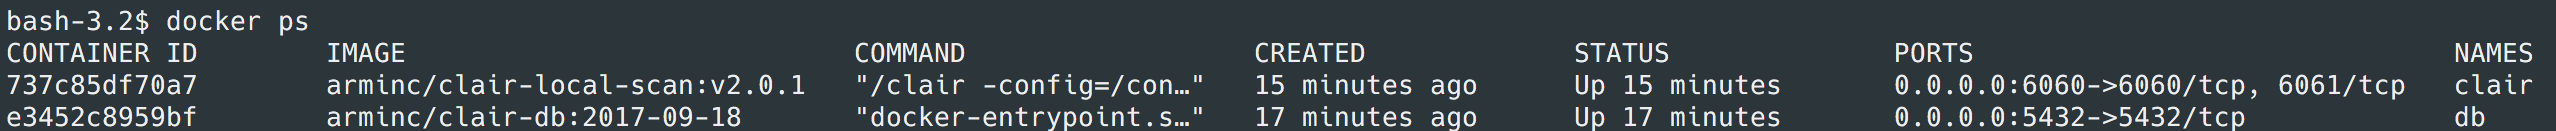
\includegraphics[width=1\textwidth]{clair_running.png}}
  \caption{Clair successfully running}
  \label{fig:clair_running}
  \end{figure}

\subsubsection{Use Of Clair Scanner}

To install Clair Scanner we need to install first Go and \textit{dep}, that is a
dependencies manager for this programming language. The scanning tool can be
downloaded directly from the GitHub page of the project and installed using the
provided Makefile, with the command ``\textit{make ensure \&\& make build}''.
\par Clair Scanner communicates directly with the Clair server previously
launched to test our containers for vulnerabilities. It is also possible to
specify a whitelist containing allowed vulnerabilities. To analyse a Docker
image we can use the command ``\textit{clair-scanner --ip OUR\_LOCAL\_IP
IMAGE\_NAME}''. In our case it will be:
\begin{lstlisting}[language=bash,breaklines]
  ./clair-scanner --ip 10.1.22.128 hmlio/vaas-cve-2014-0160 >> /Users/Carmine/Desktop/docker_scan_report.txt
\end{lstlisting}
The result of such command is showed in \myfig{\ref{fig:clair_scanner_cmd}}. It
is possible to see how each layer of the Docker image is pushed to the Clair
server, where it is analysed. In this case the image contains 234 known
vulnerabilities. Such commands produces also a report of the vulnerabilities
found, but in this case I have appended it to a new file, that I will analyse in
the next paragraph. To specify a whitelist such command must be launched with
the \textit{--whitelist=""} option, specifying the path to the whitelist file.
Such file can be a simple YAML file where the allowed vulnerabilities can be
specified for each single image or for all the Docker images to analyse.   

\begin{figure}[ht!]
  \centerline{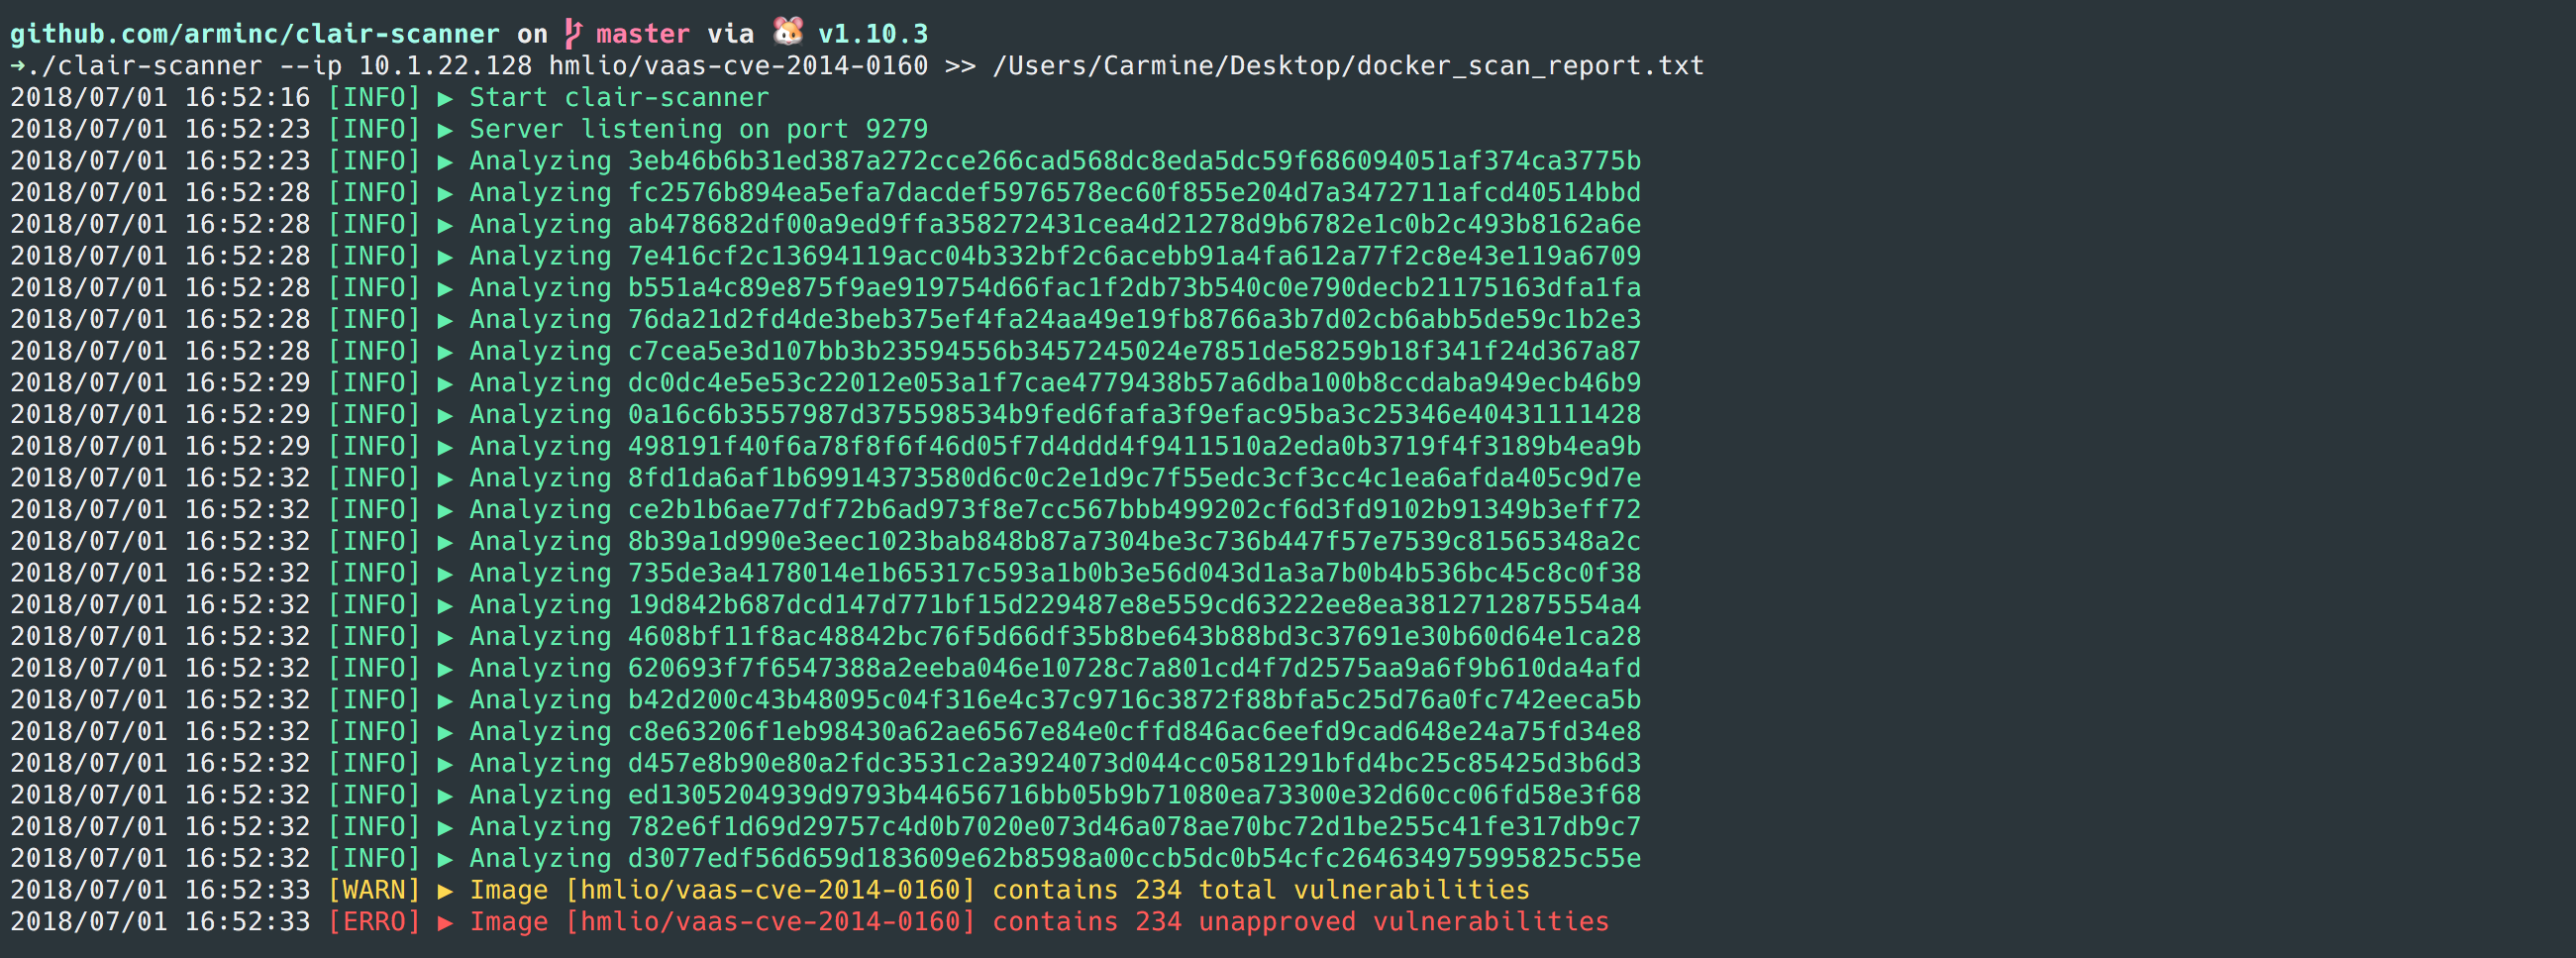
\includegraphics[width=1\textwidth]{clair_scanner_cmd.png}}
  \caption{Clair Scanner Results}
  \label{fig:clair_scanner_cmd}
  \end{figure}

\subsubsection{Results}

As stated in the previous paragraph, Clair Scanner produces a report of the
analysed image. Such report lists all the discovered vulnerabilities, ordering
them by their CVE severity. For each vulnerability is reported its CVE
identification code, the package where it was found together with the package
version and a description of the vulnerability itself. The first vulnerabilities
listed in the report of our analysed Docker image are showed in
\myfig{\ref{fig:clair_report}}.

\begin{figure}[ht!]
  \centerline{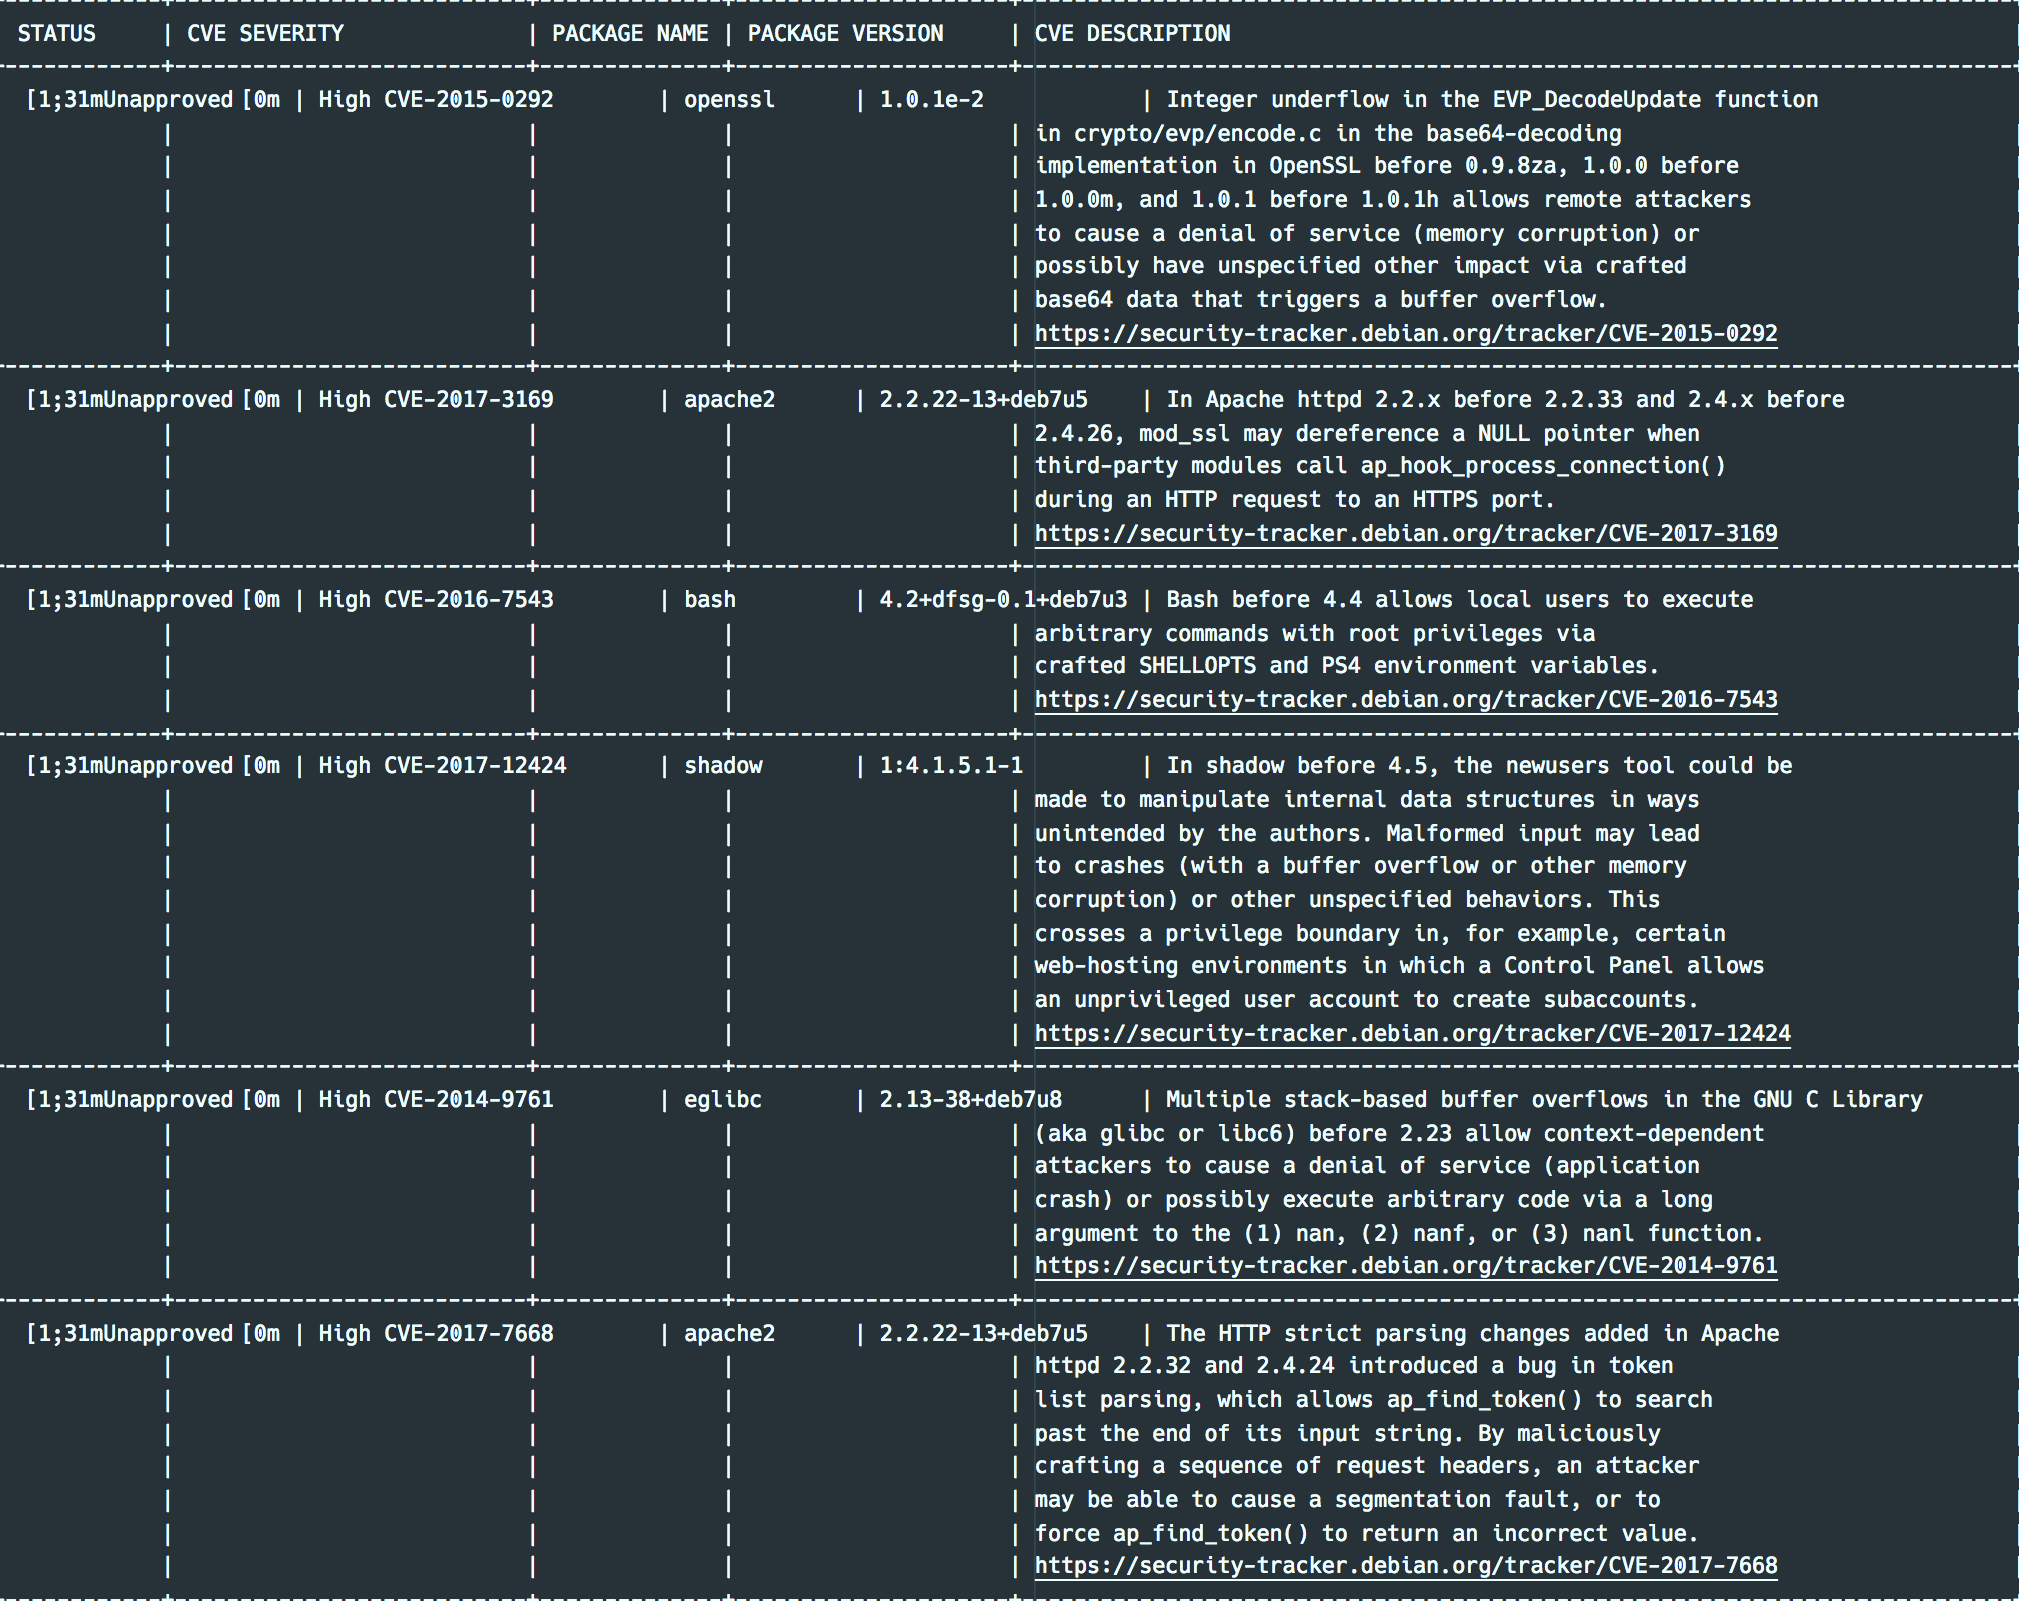
\includegraphics[width=1\textwidth]{clair_report.png}}
  \caption{Clair Scanner Report}
  \label{fig:clair_report}
  \end{figure}

We analysed the Docker image \textit{vaas-cve-2014-0160} because it contains a
version of \textit{openssl} vulnerable to \textit{heartbleed}. Clair Scanner
reports such vulnerability as can be seen in \myfig{\ref{fig:clair_heartbleed}}.

  \begin{figure}[ht!]
    \centerline{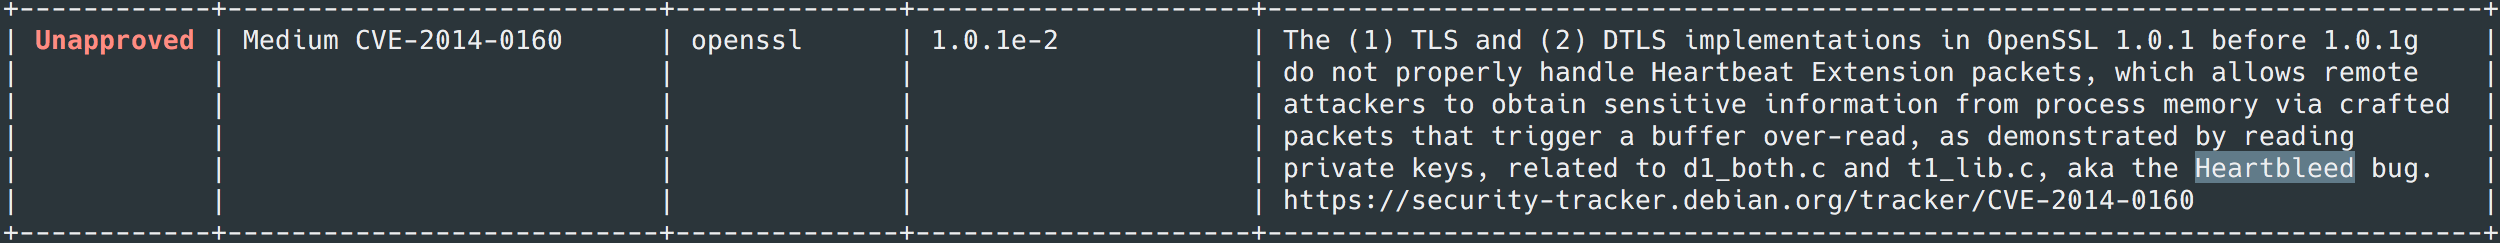
\includegraphics[width=1\textwidth]{clair_heartbleed.png}}
    \caption{Clair Scanner Report}
    \label{fig:clair_heartbleed}
    \end{figure}

\subsection{Container Monitoring}

In the previous sections we have divided Docker's security concerns into two
different types: static and dynamic. Regarding the latter we have seen how these
are related to the runtime activity of a Docker container, for example a
vulnerability not yet patched or a bug in our containerised application. \par As
seen in the previous section, the use of log mechanisms or specific tools for
monitoring container's activities can help in these contexts. In particular we
have seen how Docker offers a native system for logging and how third-party
software like Sysdig Falco can be used to actively monitor a Docker container.
We will focus on this last application, showing how it can be used in practice
to detect attacks. 

\subsubsection{Setup}

For this practical evaluation we will use a virtual machine with Debian 9.4 and
Linux Kernel 4.9.0. Falco's documentation can be found on its GitHub page
\cite{falco_doc}. It can be easily installed running the following command as
root:
\begin{lstlisting}[language=bash,breaklines]
curl -s https://s3.amazonaws.com/download.draios.com/stable/install-falco | sudo bash
\end{lstlisting}
Then it can be launched simply using the \textit{falco} command on the
terminal. \par It can be configured modifying the
\textit{/etc/falco/falco.yaml}. In particular we set it up in order to print all
the events found on \textit{/events.txt} and not on the \textit{STDOUT}, adding
the following code snippet to the configuration file:
\begin{lstlisting}[language=bash,breaklines]
syslog_output:
  enabled: false

file_output:
  enabled: true
  filename: /var/log/events.txt
\end{lstlisting}
\par As said in the first section of this research, despite a single Docker
container can be used to run multiple processes, it is a good practice to
execute just one process per container. In this way there is a better separation
of concerns, moreover this allows to know exactly which process is running
inside a certain container. This last statement can be used to enhance the
security of our system. In most attacks, in fact, the attacker that takes
control of a Docker container launches other processes inside the same
container. Using Falco we can define a rule that can be used to warn in case a
process different from the one initially defined is executed inside our
container. We can append our rule to the file
\textit{/etc/falco/falco\_rules.yaml}:

\begin{lstlisting}[language=bash,breaklines]
- rule: Unauthorised process
  desc: A process different from the defined one is spawned
  condition: spawned_process and container and container.image startswith nginx and not proc.name in (nginx)
  output: Unhautorized process (%proc.cmdline) running in (%container.id)
  priority: WARNING
\end{lstlisting}

\textit{spawned\_process}, \textit{container}, \textit{container.image
startswith} and \textit{proc.name in} are all macros defined by default in
Falco. Such conditions detect a new process that is launched in a nginx Docker
image and that is not nginx itself. Such rule also print out the name of the new
process and the ID of the involved container.

\subsubsection{Detection}

As anticipated in the definition of the Falco's rule, the Docker image that we
will use is nginx. It is one of the most popular Docker image on the Docker Hub
and it can be used to create a web server, a load balancer, a reverse proxy, ...
In our case we will just use it to launch a process from its container's
terminal. It can be launched using the command:

\begin{lstlisting}[language=bash,breaklines]
  docker run -d -P  --name falco_test nginx
\end{lstlisting}

We can verify that such container has been launched using the \textit{docker ps}
command as can be seen in \myfig{\ref{fig:nginx_launched}}, where it is also
reported the ID of the container.

\begin{figure}[ht!]
  \centerline{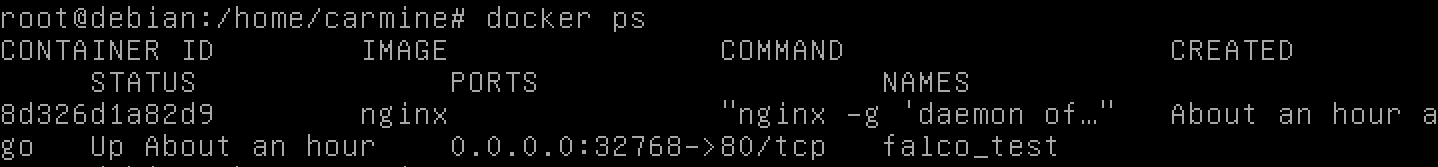
\includegraphics[width=1\textwidth]{nginx_launched.png}}
  \caption{nginx container successfully running}
  \label{fig:nginx_launched}
  \end{figure}

As said before, Falco can be simply launched using the \textit{falco} command.
It will automatically read the new configuration and the new defined rule from
\textit{/etc/falco/falco.yaml} and \textit{/etc/falco/falco\_rules.yaml}. At
this point it will be sufficient to launch from the nginx's container any
command to trigger Falco. In our case we will run the \textit{ls} command via: 
\begin{lstlisting}[language=bash,breaklines]
  docker exec -it falco_test ls
\end{lstlisting}

We can see the generated warning checking the \textit{/var/log/events.txt} file
as showed in \myfig{\ref{fig:falco_warn}}.

\begin{figure}[ht!]
  \centerline{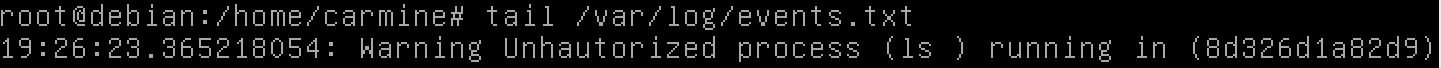
\includegraphics[width=1\textwidth]{falco_warn.png}}
  \caption{Warning from Falco}
  \label{fig:falco_warn}
  \end{figure}

\newpage

\section{Conclusions}
\label{sec:conclusions}

This research work focused on the security of Docker, in order to analyse this
software program which, despite being still ``young'', has had a great success
in the software industry. Several security threats were identified among those
described in literature, providing where possible examples of real attacks to
show how such threats are not only theoretical but also practical. These menaces
range in different field of the computer system security, from the security of
the kernel to that of the network, from aspects strictly related to the use of
Docker, such as the creation and use of images, to more general aspects
concerning the development of network services, like the management of secrets.
For each security threat one or more best practices were identified, with the
aim of creating a workflow to follow when deploying a new Docker container. Such
practices are based on the use of special configurations and ad-hoc policies or
tools, in order to increase the security of a Docker environment. Two of these
tools were also tested, demonstrating how their use can mitigate some of the
analysed threats. \par The main thesis of this research was that it is true that
Docker has become popular thanks to its ease of use, which has sped up the
development time of an application for many programmers, but it is also true
that such simplicity hides behind itself security risks. In support of this
thesis many security threats were analysed, showing how a simple \textit{docker
run} is not enough to guarantee the safety of the environment. At the same time
it is important to remark the fact that Docker is a project with relatively few
years of life and that its development is proceeding very quickly, solving in
each version released several bugs and mitigating various security threats. It
is also good to highlight the fact that Docker is an open-source project, so
anyone can contribute to its code, making it safer and speeding up its
development. Its popularity has also pushed several third-party developers to
create specific tools for it, as the ones analysed in this research. Moreover
all the best practices introduced in this work have little effect on the ease of
use of Docker, just asking for more attention and time from a developer in order
to have more security in his system. \par Docker has represented in these years
a real ``phenomenon'' in the software industry, being quickly adopted by many
companies, startups and independent programmers to sped up their development
process. Its use carries with it various security risks that should not be
ignored, but rather prevented following good practices such as those proposed in
this research. The continuous release of new tools by Docker itself and also by
third-party companies in order to address such security threats helps however to
understand the attention placed on this software program. In particular if these
new tools are able to improve the safety of Docker containers without affecting
their ease of use, the use of Docker can only continue to grow.

\newpage

\begin{thebibliography}{99}

\bibitem{docker_numbers}
About Docker, \url{https://www.docker.com/company}

\bibitem{kubernetes}
Kubernetes, \url{https://kubernetes.io/}

\bibitem{wikipedia_virtualization}
Virtualisation,
\url{https://en.wikipedia.org/wiki/Virtualization}

\bibitem{bui_docker_security}
Thanh Bui, ``Analysis of Docker Security'', January 2015

\bibitem{wikipedia_LXC}
LXC, \url{https://en.wikipedia.org/wiki/LXC}

\bibitem{red_hat_introduction_to_namespaces}
Introduction to Linux Containers,
\url{https://access.redhat.com/documentation/en-us/red_hat_enterprise_linux_atomic_host/7/html/overview_of_containers_in_red_hat_systems/introduction_to_linux_containers}
  
\bibitem{red_hat_introduction_to_cgroups}
Introduction to Control Groups (Cgroups),
\url{https://access.redhat.com/documentation/en-us/red_hat_enterprise_linux/6/html/resource_management_guide/ch01}

\bibitem{docker_official_site}
Docker official site, \url{https://www.docker.com/}

\bibitem{docker_pycon_presentation}
The future of Linux Containers, PyCon 2013,
\url{https://www.youtube.com/watch?v=wW9CAH9nSLs}

\bibitem{docker_ci_cd}
CI/CD in Docker, \url{https://www.docker.com/use-cases/cicd}

\bibitem{solomon_hyckes_wiki}
Solomon Hikes,
\url{https://en.wikipedia.org/wiki/Solomon_Hykes}

\bibitem{docker_history_wiki}
Docker History,
\url{https://en.wikipedia.org/wiki/Docker_(software)#History}

\bibitem{docker_architecture}
Docker architecture,
\url{https://docs.docker.com/engine/docker-overview/#docker-architecture}

\bibitem{docker_objects}
Docker objects,
\url{https://docs.docker.com/engine/docker-overview/#docker-objects}

\bibitem{ibm_interview_john_willis}
The most common use cases of Docker containers and organisations,
\url{https://www.ibm.com/blogs/systems/the-most-common-use-cases-of-docker-containers-and-organizations/}

\bibitem{mitigating_docker_security_issues_yasrab}
Robail Yasrab, ``Mitigating Docker Security Issues'', April 2018

\bibitem{sysdig_docker_vulnerabilities}
Seven Docker security vulnerabilities and threats,
\url{https://sysdig.com/blog/7-docker-security-vulnerabilities/}

\bibitem{red_hat_dirtycow}
CVE-2016-5195, \url{https://access.redhat.com/security/cve/cve-2016-5195} 

\bibitem{madvise_description}
MADVISE (2), \url{http://man7.org/linux/man-pages/man2/madvise.2.html}

\bibitem{dirtycow_how_it_worrks}
Demonstrating the Dirty Cow exploit,
\url{https://01.org/developerjourney/recipe/demonstrating-dirty-cow-exploit}

\bibitem{dos_wikipedia}
Denial-of-service attack,
\url{https://en.wikipedia.org/wiki/Denial-of-service_attack}

\bibitem{resource_on_docker} 
Limit a container's resources,
\url{https://docs.docker.com/config/containers/resource_constraints/}

\bibitem{docker_blog_about_container_breakout}
Docker Container Breakout Proof-of-Concept Exploit,
\url{https://blog.docker.com/2014/06/docker-container-breakout-proof-of-concept-exploit/}

\bibitem{shocker}
Shocker, \url{https://github.com/gabrtv/shocker}

\bibitem{shocker_how_it_works}
Docker breakout exploit analysis,
\url{https://medium.com/@fun_cuddles/docker-breakout-exploit-analysis-a274fff0e6b3}

\bibitem{docker_pull_red_hat}
Before you initiate a "docker pull",
\url{https://access.redhat.com/blogs/766093/posts/1976473}

\bibitem{docker_image_insecurity}
Docker Image Insecurity, \\ \url{https://titanous.com/posts/docker-insecurity}

\bibitem{CVE-2014-9357}
CVE-2014-9357, \url{https://access.redhat.com/security/cve/cve-2014-9357}

\bibitem{gummaraju_desikan_turner}
G. Jayanth, T. Desikan, Y. Turner, ``Over 30\% of Official Images in Docker Hub
Contain High Priority Security Vulnerabilities'', BanyanOps, 2015

\bibitem{privileged_accounts_managers}
What is Privileged Account Management?,
\url{https://www.coresecurity.com/blog/what-is-privileged-account-management}

\bibitem{secret_management_concerns_docker}
Secret management using Docker containers, \url{https://www.bbva.com/en/docker/}

\bibitem{ibm_data_science_experience}
IBM Data Science Experience, \url{https://datascience.ibm.com/}

\bibitem{ibm_data_sciene_report}
IBM Data Science Experience: Whole-Cluster Privilege Escalation Disclosure,
\url{https://wycd.net/posts/2017-02-21-ibm-whole-cluster-privilege-escalation-disclosure.html}

\bibitem{wiki_dsniff}
"dSniff" Wikipedia Page, \url{https://en.wikipedia.org/wiki/DSniff}

\bibitem{bogaerts_arpspoof}
ARP spoofing Docker containers,
\url{https://dockersec.blogspot.com/2017/01/arp-spoofing-docker-containers_26.html}

\bibitem{kabbe_security_docker}
J. Kabbe, ``Security analysis of Docker containers in
a production environment'', Norwegian University of Science and Technology, 2017

\bibitem{to_docker_or_not_to_docker}
T. Combe, A. Martin, R. Di Pietro, ``To Docker or Not to Docker: A Security
Perspective'', IEEE Computer Society, 2016

\bibitem{arbezzano_play_safe}
Container security and immutability,
\url{https://gianarb.it/blog/container-security-immutability}

\bibitem{mouat_using_docker}
A. Mouat, ``Using Docker. Developing and Deploying Software with Containers'',
O'Reilly Media, 2015

\bibitem{wiki_MAC}
"Mandatory access control" Wikipedia Page,
\url{https://en.wikipedia.org/wiki/Mandatory_access_control}

\bibitem{bane_jesse_frazelle}
bane, \url{https://github.com/genuinetools/bane}

\bibitem{licshield}
LiCShield, \url{https://github.com/2m4t/LiCShield}

\bibitem{licshield_paper}
M. Mattetti, A. Shulman-Peleg, Y. Allouche, A. Corradi, S. Dolev, L. Foschini,
``Security hardening of Linux containers and their workloads'', 2015

\bibitem{wiki_grsecurity}
grsecurity Page, \url{https://en.wikipedia.org/wiki/Grsecurity}

\bibitem{wiki_PAX}

Hardened/PaX Quickstart,
\url{https://wiki.gentoo.org/wiki/Hardened/PaX_Quickstart}

\bibitem{docker_secrets}
Manage sensitive data with Docker secrets,
\url{https://docs.docker.com/engine/swarm/secrets/}

\bibitem{hashicorp_vault}
What is Vault?, \url{https://www.vaultproject.io/intro}

\bibitem{hashicorp_consul}
Consul, \url{https://www.consul.io/}

\bibitem{isolate_namespace}
Isolate containers with a user namespace,
\url{https://docs.docker.com/engine/security/userns-remap/#about-remapping-and-subordinate-user-and-group-ids}

\bibitem{docker_security_scanning}
Docker Security Scanning,
\url{https://docs.docker.com/v17.12/docker-cloud/builds/image-scan/}

\bibitem{common_vulnerabilities_exposures}
Common Vulnerabilities and Exposures, \url{https://cve.mitre.org/}

\bibitem{clair}
Clair, \url{https://github.com/coreos/clair} 

\bibitem{docker_content_trust}
Content trust in Docker,
\url{https://docs.docker.com/engine/security/trust/content_trust/}

\bibitem{docker_logging_driver}
Configure logging drivers,
\url{https://docs.docker.com/config/containers/logging/configure/}

\bibitem{sysdig_falco}
Sysdig Falco, \url{https://github.com/draios/falco}

\bibitem{nyantec_network_docker}
Docker networking considered harmful,
\url{https://nyantec.com/en/2015/03/20/docker-networking-considered-harmful/}

\bibitem{kvm}
Docker KVM simple container, \url{https://github.com/BBVA/kvm}

\bibitem{zaalouk_networking}
eBPF, Microservices, Docker, and Cilium: From Novice to Seasoned,
\url{http://www.adelzaalouk.me/2017/security-bpf-docker-cillium/#security-policies-with-iptables}

\bibitem{cilium_github}
Cilium, \url{https://github.com/cilium/cilium}

\bibitem{hmlio}
hmlio/vaas-cve-2014-0160, \url{https://hub.docker.com/r/hmlio/vaas-cve-2014-0160/}

\bibitem{clair-scanner}
Clair Scanner, \url{https://github.com/arminc/clair-scanner}

\bibitem{falco_doc}
Sysdig Falco Documentation, \url{https://github.com/draios/falco/wiki}

\end{thebibliography}

\end{document}
%
% Before delivering your report, don't forget to run a spell checker, such as
% aspell (with a UK-english dictionary)
%
